\documentclass{article}
\usepackage{graphicx}
\usepackage{amsfonts}
\usepackage{amsmath}
\usepackage{amsthm}
\usepackage{url}
\usepackage{subcaption}
\usepackage[left=3cm,top=3.0cm,right=3cm,bottom=3.0cm]{geometry}

\newtheorem{theorem}{Theorem}[section]
\newtheorem{remark}{Remark}
\newcommand{\norm}[1]{\left\lVert#1\right\rVert}

\title{Newton-Krylov Methods for Computing Steady States of Particle Timesteppers via Optimal Transport}
\author{Hannes Vandecasteele, Nicholas Karris, Alexander Cloninger, Ioannis G. Kevrekidis}
\date{\today}

\begin{document}
\maketitle

\begin{abstract}
Timesteppers are a cornerstone of computational science and engineering. Though they are typically used to advance the system forward in time, they can also be viewed as nonlinear mappings that implicitly encode steady states and stability information. In this work, we extend the matrix-free framework for calculating steady states from deterministic systems to stochastic particle simulations, where intrinsic randomness prevents direct steady state extraction. By formulating stochastic timesteppers in the language of optimal transport, we reinterpret them as operators acting on probability measures rather than on individual trajectories. This perspective enables the construction of smooth cumulative- and inverse-cumulative-distribution-function ((I)CDF) timesteppers that evolve distributions rather than particles. Combined with matrix-free Newton–Krylov solvers, these smooth timesteppers allow for efficient computation of steady-state distributions even under high stochastic noise. We perform a detailed error analysis quantifying how noise affects finite-difference Jacobian approximations, and demonstrate that convergence can be obtained even in the high noise regime. Finally, we introduce higher-dimensional generalizations based on smooth CDF representations of particles, and validate its performance on a non-trivial two-dimensional distribution. Together, these developments establish a unified, variational framework for computing steady states of both deterministic and stochastic timesteppers.
\end{abstract}

\section{Introduction}
Timesteppers are the backbone of modern computational science. Given the state $u(t)$ of our system at time $t$, i.e., a function or a collection of particles, and a time horizon $T$, a timestepper $\phi_{T}$ advances the state forward in time
\begin{equation}
    u(t+T) = \phi_{T}\left(u(t)\right),
\end{equation}
so that iterating the map generates a trajectory $\{u\left(n T\right)\}_{n=0}^\infty$. When the timestepper is stable, the limit of $u\left(nT\right)$ approximates the steady-state solution of the underlying model. In the context of this manuscript, this model will typically a differential equation of some kind. In the traditional viewpoint, timesteppers are used naively: we apply $\phi_{T}$ repeatedly to obtain a numerical trajectory that is then studied for qualitative and quantitative convergence features. This is still the dominant approach in numerical analysis, computational science, and simulation software across physics, chemistry, and engineering.

However, timesteppers can also be used much more intelligently. They contain everything about the problem, namely the underlying differential equation, the model parameters, and the boundary conditions. Instead of treating them only as simulators, one may ask what information about the system can be extracted directly from the timestepper mapping itself. Several important system-level tasks can be formulated in this way
\begin{itemize}
\item[1.] Steady states. Fixed points $u^* = \phi_{T}\left(u^*\right)$ of the timestepper correspond to the steady (or invariant) states of the underlying differential equation.
\item[2.] Eigenvalues and Stability. The Jacobian $J = D\phi_{T}(u^*)$ of the timestepper at $u^*$ contains all spectral information from which eigenvalues and stability properties of the underlying model can be inferred. There is a direct relationship between the eigenvalues of the timestepper and the eigenvalues of the right-hand side of the differential equation.
\item[3.] Control and identification. By systematically tracking the steady-state solutions across varying parameter values, we can trace the corresponding solution branches and identify critical points where the system’s behavior changes drastically, such as folds, bifurcations, or Hopf bifurcations.
\end{itemize}
A convenient way to unify these three tasks is through the residual mapping
\begin{equation} \label{eq:psi}
    \psi(u) = u - \phi_{T}\left(u\right)
\end{equation}
This formulation for calculating steady states allows us to apply the full machinery of iterative nonlinear solvers through matrix-free methods. Particularly, in previous work~\cite{}, we used the Newton-Krylov and Arnoldi methods to calculate steady-state profiles and the leading eigenvalues of the Jacobian respectively. These methods are matrix-free. We do not need explicit Jacobian matrices to compute the steady state or the leading eigenvalues. This last part is essential because codes implementing a timestepper rarely have their Jacobians coded as well. Even if they do so in the form of hand-coded formulas or automatic differentiation, evaluating the (typically large) Jacobian is too time-consuming and uses a lot of memory. Matrix-free methods avoid these bottlenecks by approximating the action of the Jacobian $D \psi(u) \cdot v$ in a particular direction $v$ on the fly using finite differences
\begin{equation} \label{eq:JVP}
    D \psi(u) \cdot v \approx F(u, v) = \frac{\psi(u + \varepsilon v) - \psi(u)}{\varepsilon}.
\end{equation}
Although this approximation induces an error, it is typically negligible compared to the speedups that can be obtained.

In our previous work, we focused on deterministic timesteppers, developing Newton–Krylov and other matrix-free methods to compute steady states and stability information directly from the mapping $\psi(u)$. This line of research established how timesteppers could serve as fixed-point solvers for macroscopic equations, particularly in gradient systems where convergence is theoretically guaranteed. In the present work, we expand this framework to stochastic settings, where timesteppers are no longer deterministic mappings of states but rather involve random evolutions of particle ensembles. Here, the naive formulation $X - \phi_{T}(X) = 0$ for a particle ensemble $X$ is ill-defined since particles do not carry one-to-one correspondences across time steps. Furthermore, even in steady state, particles typically fluctuate because of thermal noise. This does not mean a steady state distribution of stochastic particles does not exist, only that the mathematical equality $X = \phi_T(X)$ does not hold.

Optimal Transport (OT) solves this difficulty by providing a principled way to compare ensembles in a Wasserstein space, enabling the construction of well-defined particle-based timesteppers. This extension allows us to treat both deterministic and stochastic dynamics within a unified variational framework. From an optimal transport perspective, we treat the evolving distribution of particles as a time dependent probability measure $\mu_t$ on $\mathbb{R}^d$, rather than trying to follow each particle individually. If $\mu_t$ is ``smooth'' in the sense of having a density and evolving in a regular way, then there is a velocity field $v_t$ such that the continuity equation
\begin{equation} \label{eq:OTcontinuity}
\partial_t \mu_t + \nabla \cdot (v_t \mu_t) = 0
\end{equation}
describes how mass flows. The minimal energy (and smoothest) velocity field $v_t$ can be computed via the optimal transport map $T_{\mu_t}^{\mu_{t+h}}$
\[v_t = \lim_{h\to 0}\frac{T_{\mu_t}^{\mu_{t+h}} - Id}{h}.\]
We have previously shown that under certain assumptions on the smoothness of $(\mu_t)_{t\ge 0}$, forward Euler methods using $v_t$ are first order accurate in $W_2$ \cite{karris2024using}.

The key advantage over tracking particles individually (which in stochastic or chaotic systems can be very noisy) is that this optimal transport based method aggregates the motion of \emph{mass} rather than individual sample paths. In many systems, especially those with fast / slow scales, individual particle trajectories will jitter, be non-differentiable, or otherwise provide a noisy or misleading picture at short time scales. By contrast, the distribution $\mu_t$ often changes in a much smoother and more coherent manner. By fitting the velocity field from optimal transport between successive empirical distributions, one effectively filters out the microscopic stochasticity and focuses on how the bulk of the particles move. This produces a cleaner signal, which will allow for a more accurate Newton-Krylov step.

These optimal transport algorithms are especially efficient in one dimension. In fact, the optimal transport map of a set of particles can be obtained simply by sorting the particles. Additionally, there are direct links to the theory of probability distributions. Computing the cumulative density function (CDF) of a set of particles, and then immediately applying the inverse cumulative density function (ICDF) will result in the OT map of the original particles~\cite{}. The advantage of the CDF/ICDF formulation is that inverse CDFs are always smooth, which allows us to employ advanced optimization techniques for calculating steady states of particle systems. Indeed, a smooth macroscopic ICDF-to-ICDF timestepper can be built directly in three steps: 1) Sample the ICDF by evaluating it in percentiles; 2) Propagate the particles using the stochastic timestepper; 3) Compute the new ICDF from the particle locations. This scheme gives us a bridge between microscopic particle simulations and macroscopic evolution.

However, real-world systems are multi-dimensional, and the inverse cumulative density function is not defined in higher dimensions. The regular cumulative density function does carry over to multiple dimensions, so we can construct a CDF-to-CDF timestepper using the same three steps: 1) Generate samples from the multidimensional CDF; 2) Propagate the particles using the stochastic timestepper; 3) Compute the new CDF from the particles. However, the first step becomes nontrivial in multiple dimensions because simply inverting the CDF at `percentiles' for sampling is impossible. We need to project the multidimensional CDF down to its one-dimensional representations to generate samples. One such technique is to use marginal and conditional CDFs. First, we construct the marginal CDF in the first dimension and generate $x$-samples from this 1D CDF by inverting it. Then, for every 1D sample, we construct the conditional CDF of the second dimension $y$ and invert it. Classical constructions such as the Knothe–Rosenblatt rearrangement allow for the extension of 1D CDF concepts into higher dimensions, though at the cost of introducing asymmetry. More modern approaches based on sliced optimal transport offer a flexible alternative, projecting the problem onto many one-dimensional slices before reassembling the results. Both types of “tricks”—the old and the new—are crucial in making OT-based timesteppers practical for complex and higher-dimensional systems.

Having reinterpreted stochastic timesteppers in optimal transport terms, we can now deploy advanced numerical solvers to compute steady-state distributions. However, there is one computational roadblock. The (I)CDF-to-(I)CDF timestepper is itself stochastic because it is built around a particle timestepper. Averaging over independent runs or variance reduction might reduce this stochastic variability, but evaluations of $\psi$ will always be non-deterministic. Indeed, if we evaluate $\psi$ in $u + \varepsilon v$ and $u$ independently, with the respective stochastic error terms $\xi_1$ and $\xi_2$, we have effectively calculated $\tilde{\psi}(u) = \psi(u) + \xi_1$ and $\tilde{\psi}(u + \varepsilon v) = \psi(u+ \varepsilon v) + \xi_2$. The Jacobian-vector product in equation~\eqref{eq:JVP} then becomes
\begin{equation} \frac{\tilde{\psi}(u+\varepsilon v) - \tilde{\psi}(u)}{\varepsilon} = \frac{\psi(u+\varepsilon v) + \xi_2 - \psi(u) - \xi_1}{\varepsilon} = F(u, v) + \frac{\xi_2 - \xi_1}{\varepsilon}.
\end{equation}
At first sight, the error in the finite-difference approximation of the Jacobian looks catastrophic. Indeed, since $\xi_1$ and $\xi_2$ are independent (and we can assume the same error distribution), the variance of $\xi_2-\xi_1$ is double that of $\xi_1$. We further divide it by a (typically) small step size $\varepsilon$! To keep the stochastic error within reasonable limits, we must use a large $\varepsilon$, which in turn induces a larger approximation error in~\eqref{eq:JVP}. In this paper, we will connect the existing error analysis of the (stochastic-free) Newton-Krylov method, and particularly of the Jacobian-vector products, with this stochastic error. We will demonstrate, both theoretically and numerically, that one can still compute steady-state (I)CDFs of stochastic systems accurately, up to a certain noise level or tolerance. We will also demonstrate numerically that the `optimal' finite difference step size $\varepsilon$ increases from $10^{-8}$ to $10^{-2}$ -- $10^{-1}$ in double precision.

\paragraph{Contributions of this work}
This work extends the timestepper-based framework for steady-state computation from deterministic to stochastic particle systems by combining matrix-free Newton–Krylov methods with optimal transport formulations. Our main contributions are as follows:
\begin{itemize}
    \item[1.] \textbf{Generalization of timestepper-based fixed-point computation to stochastic systems.} We extend the classical residual formulation $\psi(u) = u - \phi_T(u)$ to stochastic particle timesteppers, where individual particle mappings are ill-defined due to randomness.
    \item[2.] \textbf{Formulation of stochastic timesteppers in the language of Optimal Transport.} We reformulate timesteppers as operations acting on probability measures, and use the Wasserstein distance to define a well-posed residual that is minimized in steady state.
    \item[3.] \textbf{Development of smooth distribution-based timesteppers.} We develop smooth (I)CDF-to-(I)CDF timesteppers that bridge stochastic simulations with distributional evolution, enabling the use of higher-order optimization such as the Newton-Krylov method.
    \item[4.] \textbf{Error analysis of Newton–Krylov methods in the stochastic setting.}  We extend the theoretical error analysis of the Newton-Krylov method to include stochastic timesteppers, providing a quantitative trade-off between finite-difference step size and the number of stochastic particles.
    \item[5.] \textbf{Efficient extensions to higher dimensions.} We propose two practical multidimensional generalizations: a CDF-to-CDF timestepper based on marginal and conditional CDFs, and a sliced Wasserstein formulation relying on one-dimensional projections.
    \item[6.] \textbf{Numerical validation and demonstrations.} We demonstrate the performance of the proposed methods on important stochastic systems, including a two-dimensional distribution, highlighting accuracy and robustness of Newton--Krylov on smooth representations of particle distributions.
\end{itemize}

\paragraph{Outline of the Manuscript}
We start this paper in section~\ref{sec:trajectories} by discussing how steady-state distributions of potential systems can be obtained from simulation trajectories by directly estimating the local velocity field. We also explain why this approach cannot work for non-potential systems. Next, in section~\ref{sec:nk} we introduce the matrix-free Newton-Krylov method. We perform a general error analysis in the non-stochastic case and demonstrate convergence of Newton-Krylov on the mean-field equation associated to particle methods. We also discuss how the integration time horizon $T$ can be optimally chosen through a spectral analysis of the timestepper. Afterwards, we move on to stochastic timesteppers in section~\ref{sec:w2_stochastics}. In particular, we focus on first-order (gradient-based) optimizers for finding steady-states through a reformulation of~\eqref{eq:psi} using the Wasserstein distance. We demonstrate, theoretically and numerically on three examples, that this Wasserstein optimization scheme converges quickly and smoothly to the correct steady-state particle distribution. We also perform an extended error analysis of the Newton-Krylov method in the stochastic case (see section~\ref{subsec:nk_noisy} and prove that second-order optimizers applied to this Wasserstein formulation suffer from large noise errors. This result motivates us to investigate smooth representations of particle distributions, and in particular the ICDF-to-ICDF timestepper in section~\ref{sec:particles_to_smooth}. We explain the main idea in detail and demonstrate improved convergence of the Newton-Krylov method using these smooth representations. Finally, in Section~\ref{sec:higher_dimensions}, we discuss two alternative smooth representations for higher-dimensional systems: the CDF-to-CDF timestepper and its equivalent sliced Wasserstein formulation. We then demonstrate their effectiveness on a two-dimensional half-moon probability distribution. We conclude this paper with a summarizing discussion and outlook for further research in section~\ref{sec:conclusion}.

\section{Steady-State Distributions from Trajectories} \label{sec:trajectories}
The OT timestepper approximates the dynamics of an evolving density $\mu_t(t)$ by transporting an ensemble of particles forward in time and reordering the output particles using the OT map. Formally, let $X=\{X_i\}_{i=1}^N$ be a particle ensemble at time $t$ and let $\phi_{T}$ be the stochastic particle integrator over a short horizon $T$. Then, from the output ensemble $Y=\{Y_i\}_{i=1}^N$
\begin{equation}
    Y = \phi_{T}(X),
\end{equation}
we can obtain a first-order approximation of the local (in time) velocity field $v_t$ through
\begin{equation} \label{eq:OT_Euler}
    \frac{T_X^Y(Y) - X}{T} \approx v_t(X).
\end{equation}
Here, $T_X^Y(X)$ is the optimal-transport mapping from $X$ to $Y$. Assuming that the velocity field $v(x)$ is constant over time, the steady-state distribution $\mu(x) = \mu_{\infty}(x)$ can be obtained by solving the linear steady-state equation
\begin{equation} \label{eq:ss_velocity_invariant}
    \nabla \cdot \big(v(x)\mu(x)\big) = 0.
\end{equation}
Equivalently, $\mu$ is constant along the streamlines of $v(x)$. For gradient systems with $v(x) = -\nabla U(x)$, this immediately reduces to the familiar Boltzmann-Gibbs measure
\begin{equation} \label{eq:boltzmann-gibbs}
    \mu(x) \propto \exp(-\beta U(x)),
\end{equation}
where $\beta$ is typically the inverse temperature of the system.

Using the Euler-OT timestepper, the velocity field $v(x)$, the potential $U(x)$ and the invariant distribution $\mu(x)$ can all be obtained by doing well-initialized short bursts of simulation. Mathematically, for small $\Delta t$, the increments of the particles satisfy
\begin{equation}
 Y_n - X_n \sim \mathcal{N}\big(-\nabla U(X_n)\Delta t,\; 2\beta^{-1}\Delta t I\big). \label{eq:traj}
\end{equation}
Reordering of the particles using the OT mapping ensures that $X_n$ and $Y_n$ stay close, even under large random Brownian increments. This OT step ensures an accurate approximation of the local velocity field $v(X_n)$. Next, we approximate the potential by a linear combination of basis functions
\begin{equation}
 U(x) \approx U_\theta(x) = \sum_{j=1}^p \theta_j \psi_j(x),
\end{equation}
with gradient
\begin{equation}
 \nabla U_\theta(x) = \sum_{j=1}^p \theta_j \nabla \psi_j(x).
\end{equation}
The parametric maximum-likelihood estimator for $\theta$ is
\begin{equation}
 \theta^* = \arg\min_\theta -\frac{\beta}{4\Delta t}\frac{1}{N}\sum_{n=1}^N \bigg\| Y_n - X_n + \Delta t \sum_{j=1}^p \theta_j \nabla\psi_j(X_n) \bigg\|^2, \label{eq:mle}
\end{equation}
which reduces to a linear system of equations
\begin{equation}
 G_N\theta^* = b_N,
\end{equation}
defined by the matrix $G_N$ and right hand side $b_N$
\begin{align}
 G_N &= \frac{1}{N}\sum_{n=1}^N \nabla \psi(X_n)\nabla\psi(X_n)^T, \\
 b_N &= -\frac{1}{N}\sum_{n=1}^N \nabla \psi(X_n)\frac{Y_n - X_n}{\Delta t}.
\end{align}

\paragraph{Example of a Gradient System} As an example, consider the bimodal distribution given by potential energy
\begin{equation}
    U(x) = \frac{1}{2}\left(x^2 - 1\right)^2.
\end{equation}
We use the procedure outlined above to estimate the invariant bimodal distribution. For the basis $\psi_j(x)$ we take $51$ radial basis functions equidistant between $-4$ and $4$ with standard deviation $\sigma = 0.2$, i.e.
\begin{equation}
    \psi_j(x) = \exp\left(-\frac{(x - x_j)^2}{2 \sigma^2}\right), \ \ x_j = -4 + 0.16 j.
\end{equation}
To obtain a globally accurate estimate of the velocity field, we initialize $N=10^5$ particles uniformly between $-4$ and $4$ and propagate them through the Euler-OT timestepper. Figure~\ref{fig:BimodalFlow} shows the least-squares fit on the analytic velocity field and the steady-state distribution. A boundary artifact near $x=-4$ and $x=4$ in the estimated velocity field arises because the radial basis functions converge to $0$ for large $x$, but the Euler-OT estimated velocity field matches the true velocity field well in the bulk of the domain.

\begin{figure}
    \centering
    \begin{subfigure}[b]{0.5\textwidth}
        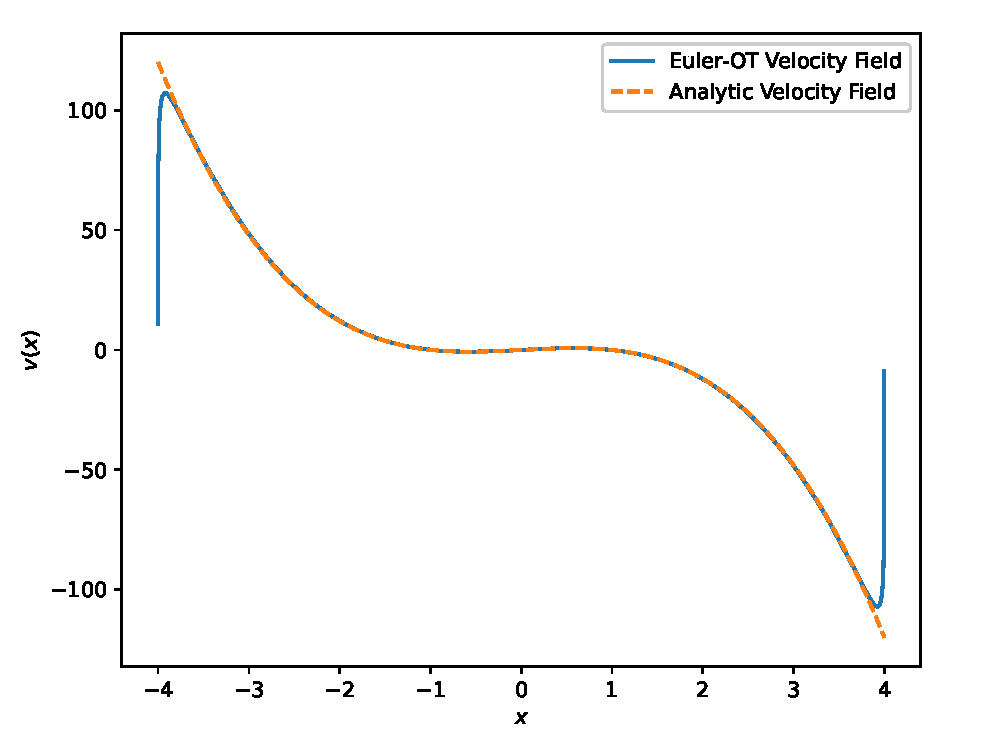
\includegraphics[width=\textwidth]{figures/BimodalFlowVelocityField.eps}
    \end{subfigure}%
    \begin{subfigure}[b]{0.5\textwidth}
        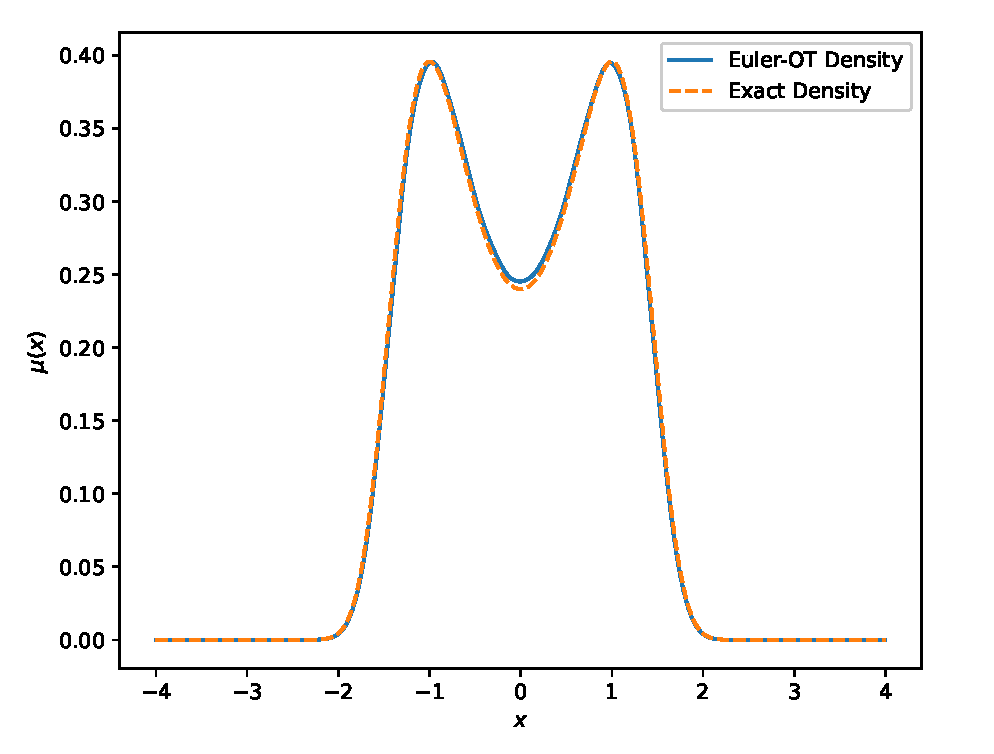
\includegraphics[width=\textwidth]{figures/BimodalFlowDensity.eps}
    \end{subfigure}
    \caption{Left: Estimated velocity field $v(x)$ using the Euler-OT method (blue) versus the analytic velocity field $-\nabla U(x)$ (dashed orange). Right: Corresponding estimated steady-state distribution (blue) compared to the analytic steady-state distribution (dashed orange).}
    \label{fig:BimodalFlow}
\end{figure}

\paragraph{Example of a non-Gradient System}
This procedure of estimating the invariant distribution using the Euler-OT timestepper does not work anymore for non-gradient systems because the velocity field is not necessarily time-independent [\textbf{Theory needed here!!}]. As an example, consider the SDE
\begin{equation} \label{eq:nonlinear_flow}
    dX_t = (1 + X_t^2)dt + \sqrt{1+X_t^2} dW_t.
\end{equation}
In this model, the noise variance $\sigma(x)^2 = 1+x^2$ is of the same size as the drift $b(x)=1+x^2$, so trajectories will diverge arbitrarily far from the bulk before returning. However, the process~\eqref{eq:nonlinear_flow} still has a steady-state distribution
\begin{equation}
    \mu(x) \propto \frac{e^{2 \arctan(x)}}{(1+x^2)^2}
\end{equation}
Furthermore, by matching this steady-state distribution with equation~\eqref{eq:boltzmann-gibbs}, we can obtain an effective potential energy $\tilde{U}(x) = -\log \mu(x)$. However, the (possibly time-dependent) velocity field $v_t(x)$ does not correspond to $-\nabla \tilde{U}(x)$ because the trajectories of the original model~\eqref{eq:nonlinear_flow} are not the same as those of the overdamped Langevin dynamics
\begin{equation*}
    dY_t = -\nabla \tilde{U}(Y_t)dt + \sqrt{2} d\tilde{W}_t
\end{equation*}
where $\tilde{W}_t$ is a Brownian motion independent from $W_t$~\eqref{eq:nonlinear_flow}.

Figure~\ref{fig:NonlinearFlow} shows how the Euler-OT estimated velocity field, for all intents and purposes, the `true' velocity field, differs from the negative effective potential gradient. We also show how the resulting estimated steady-state differs from the true invariant distribution because the velocity field is not constant over time and equation~\eqref{eq:ss_velocity_invariant} no longer holds.

\begin{figure}
    \centering
    \begin{subfigure}[b]{0.5\textwidth}
        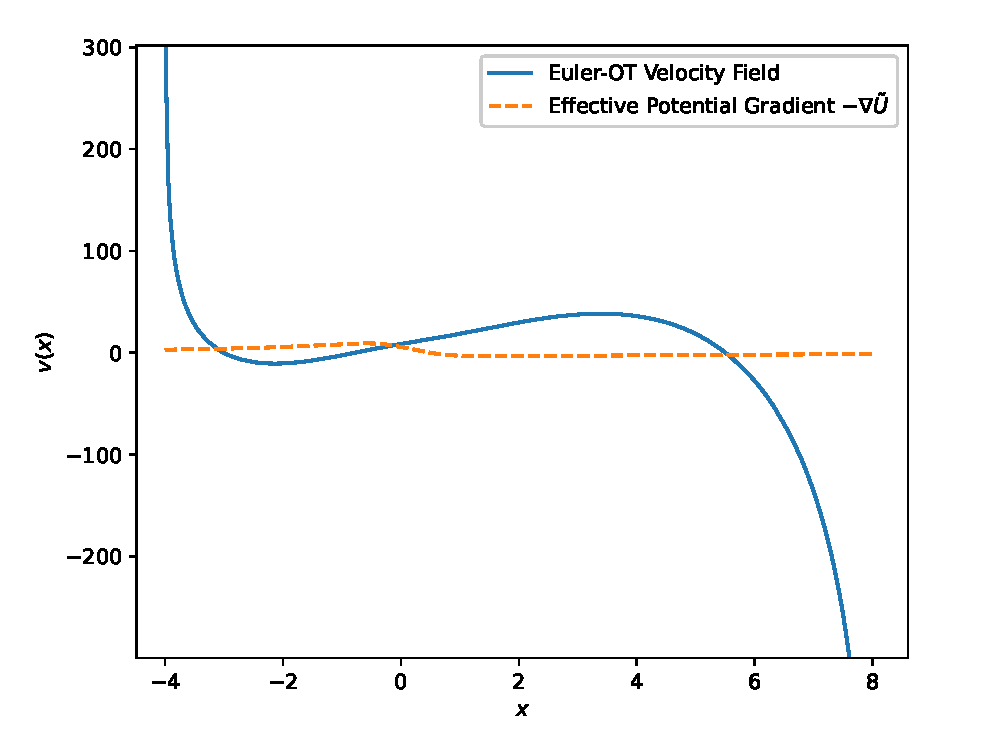
\includegraphics[width=\textwidth]{figures/NonlinearFlowVelocityField.eps}
    \end{subfigure}%
    \begin{subfigure}[b]{0.5\textwidth}
        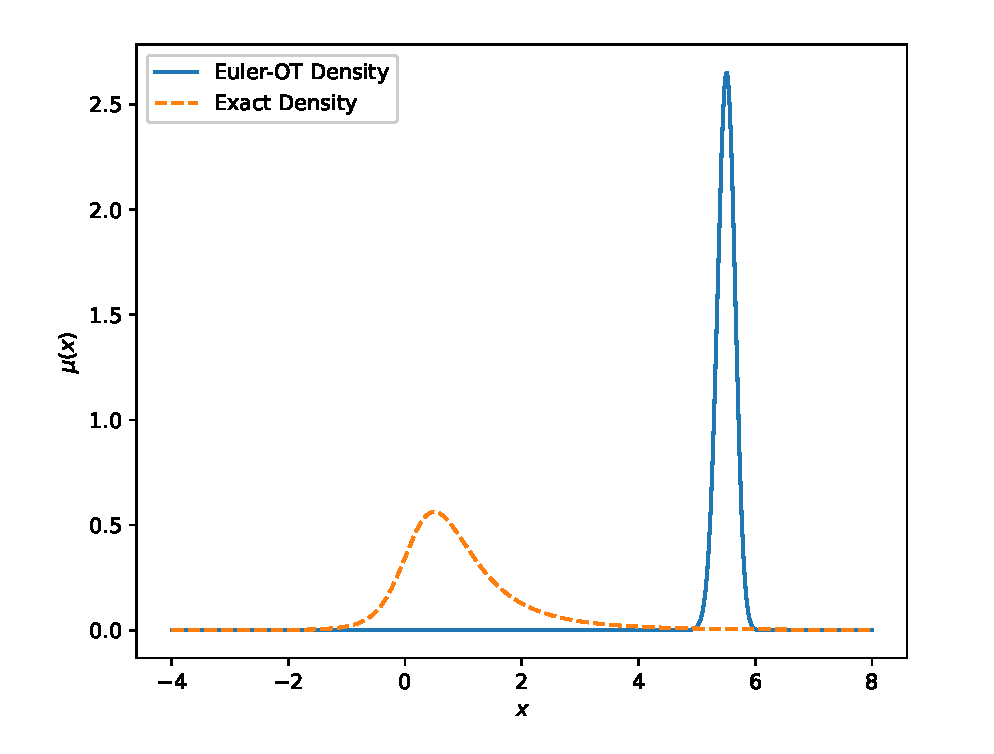
\includegraphics[width=\textwidth]{figures/NonlinearFlowDensity.eps}
    \end{subfigure}
    \caption{Left: Estimated velocity field $v(x)$ using the Euler-OT method (blue) versus the effective energy gradient $-\nabla \tilde{U}(x)$ (dashed orange). Right: Corresponding Euler-OT estimated steady-state distribution (blue) compared to the analytic steady-state distribution (dashed orange).}
    \label{fig:NonlinearFlow}
\end{figure}

These numerical results indicate that we need a more general and systematic procedure for obtaining steady-state profiles from the Euler-OT timestepper. We propose using the Newton-Krylov method on smooth representations of the particle timestepper for precisely this purpose. We outline the Newton-Krylov framework in section~\ref{sec:nk} and provide a structured error analysis for stochastic timesteppers.

\section{Newton--Krylov Framework} \label{sec:nk}
The main idea behind the Newton-Krylov method is to approximate the Jacobian of the objective function, $\nabla \psi(u_k)$, using finite differences with step size $\varepsilon$
\begin{equation} \label{eq:fd_2}
    D \psi(u_k) \cdot v \approx F(u_k, v) = \frac{\psi(u_k + \varepsilon v) - \psi(u_k)}{\varepsilon}.
\end{equation}
Since this matrix-free formulation can only approximate matrix-vector products, and not the full Jacobian directly, we must use iterative Krylov methods to solve the linear system
\begin{equation} \label{eq:linear_newton}
    D\psi(u_k) s_k = -\psi(u_k)
\end{equation}
to obtain the next Newton guess $u_{k+1} = u_k + s_k$. Because the Jacobian is not generally symmetric, we will use the GMRES method for solving~\eqref{eq:linear_newton}.

The authors of~\cite{} performed an extensive error analysis of the Newton-Krylov method; we will repeat their main findings here. There are three main sources of error in the Newton-Krylov method: (1) approximation and rounding errors in the approximate Jacobian~\eqref{eq:fd_2}, (2) tolerance $\eta_k$ used to solve~\eqref{eq:linear_newton}, and (3) rounding errors in other calculations in addition to these. Each of these errors can be controlled. Indeed, one typically uses $\varepsilon \sim \mathcal{O}\left(\sqrt{\varepsilon_{\text{mach}}}\right)$ where $\varepsilon_{\text{mach}} = 2.2 \ 10^{-16}$ is the machine precision in double precision floating point arithmetic. This limits the first error contribution to the same bound of $\mathcal{O}\left(\sqrt{\varepsilon_{\text{mach}}}\right)$. For the second error contribution, the authors of~\cite[Theorem 2.12]{} proved that if the sequence of GMRES tolerances $\eta_k$, defined such that
\begin{equation}
    \norm{D\psi(u_k) s_k + \psi(u_k)} \leq \eta_k \norm{\psi(u_k)}
\end{equation}
decreases to $0$, then the Newton-Krylov method converges linearly to the exact root of $\psi$, i.e., $u_k \to u_{\infty} = u^*$ where $u^*$ is the exact solution. Their analysis remains true whenever the approximation and rounding errors in~\eqref{eq:fd_2} remain minimal; that is, they are of order $\mathcal{O}\left(\sqrt{\varepsilon_{\text{mach}}}\right)$.

Of course, in practice, the tolerances $\eta_k$ do not decrease in subsequent nonlinear Newton-Krylov iterations; rather, they remain constant $\eta_k = \eta$ for all $k \geq 1$. In this case, the Newton-Krylov method will always make a deterministic error of size
\begin{equation} \label{eq:backward_nk_error}
    \norm{\psi(u_\infty)} \leq C\left( \sqrt{\varepsilon_{\text{mach}}} + \limsup_{k} |\eta_k| + \varepsilon_{\text{mach}}\right).
\end{equation}
This result can be proven as a consequence of Theorem 2.12 in~\cite{}. Here, $C$ is a constant independent of $\varepsilon_{\text{mach}}$ and $\eta_k$ but not of $\psi$ and $T$. The final term in equation~\eqref{eq:backward_nk_error} of $\varepsilon_{\text{mach}}$ is due to (3): general rounding errors in the remaining calculations. Finally, since the condition number of a simple root is $\norm{D\psi(u^*)^{-1}}$, we also obtain a bound for the forward error
\begin{equation}
 \norm{u_\infty - u^*} \leq C \norm{D\psi(u^*)^{-1} }\left( \sqrt{\varepsilon_{\text{mach}}} + \limsup_{k} |\eta_k| + \varepsilon_{\text{mach}} \right)
\end{equation}
in floating point arithmetic.

\subsection{Determining $T$ from the Spectral Gap}
Beyond our Newton–Krylov error analysis, it is instructive to examine how information about steady state $u^*$ is encoded in timestepper $\phi_T$ and residual $\psi(u) = u-\phi_T(u)$. Linearization of the PDE
\begin{equation}
    \partial_t u_t = f(u_t)
\end{equation}
around $u^*$ gives $J = D f(u^*)$ with eigenvalues $\lambda_i$. This linearization of the flow map $\phi_T$ is then $D \phi_T(u^*) = \exp\left(T J\right)$ so that
\begin{equation}
    D \psi(u^*) = I - \exp\left(T J\right)
\end{equation}
This mapping transfers the continuous-time stability spectrum of $f$ into a discrete-time residual spectrum: eigenvalues with $\operatorname{Re}\lambda_i \approx 0$ (slow or neutral modes) yield $|\mu_i|\approx 0$, while strongly damped modes $(\operatorname{Re}\lambda_i \ll 0)$ are pushed toward $|\mu_i|\approx 1$.  As $T$ increases, a clear spectral gap typically opens between these two clusters.  Choosing $T$ too small leaves the modes entangled; choosing it too large pushes all $\mu_i$ towards $1$ and degrades conditioning. The optimal integration window therefore balances the resolution of slow modes with numerical stability and cost.

Let $u$ be the current Newton-Krylov guess, a point close to the steady-state solution $u^*$. It is safe to say that the eigenvalues and eigenvectors of $D\phi_T(u)$ will not deviate from $\lambda_i$ and $v_i$ respectively too much. Also let $\lambda_1$ be the eigenmode corresponding to the dominant, near steady-state dynamics. For a stable PDE solution, this means $0 > \text{Re}(\lambda_i) > \text{Re}(\lambda_i)$ for all $i > 1$. By perturbing the current solution $u$ in the direction of $v = \sum_{i=1}^n a_i v_i$, the flow map $\phi_T(u)$ will change in the first order by
\begin{equation} \label{eq:Jac_expansion}
    D \phi_T(u) v = D \phi_T(u) \left(\sum_{i=1}^n  a_i \phi_T(u) v_i \right) = \sum_{i=1}^n a_i \exp(T \lambda_i) v_i,
\end{equation}
where we used the fact that $v_i$ are (approximate) eigenvectors of $D\phi_T(u)$. In this expansion, the factor $\exp(T \lambda_1)$ will be larger than all other $\exp(T \lambda_i)$ in real part. Similar to the analysis of the power iteration, the above expansion can be rewritten as the dominant term plus high-frequency corrections
\begin{equation}
     D \phi_T(u) v =  \exp(T \lambda_1)\left(a_1 v_1 + \sum_{i=2}^n a_i \frac{\exp(T \lambda_i)}{ \exp(T \lambda_1)} v_i \right).
\end{equation}
When the integration time $T$ is large enough, the other terms in this expansion will be small compared to the first term $\exp(T \lambda_1) a_1 v_1$, which represents the steady state solution. 

To ensure that the Newton–Krylov method can discern meaningful descent information from the Jacobian $D\phi_T(u) v$, rather than being dominated by high-frequency `noise' from the remaining terms in~\eqref{eq:Jac_expansion}, a high signal-to-noise ratio is required. Mathematically, we require
\begin{equation}
    \left|\frac{\exp(T \lambda_i)}{\exp(T \lambda_1)} \right|\ll 1
\end{equation}
and this provides a criterion for choosing the minimal integration time $T$. Defining the signal-to-noise ratio as $1/\eta$ with $\eta \ll 1$, we desire
\begin{equation*}
    \exp\left(T \left(\text{Re}(\lambda_i) - \text{Re}(\lambda_1)\right)\right) \leq \eta
\end{equation*}
 for all $i > 1$, and therefore
\begin{equation}
    T \geq \frac{\ln \eta}{\text{Re}(\lambda_2) - \text{Re}(\lambda_1)}
\end{equation}
because $\text{Re}(\lambda_i) \leq \text{Re}(\lambda_2) < \text{Re}(\lambda_1) < 0$. In practice, we typically want a signal-to-noise ratio of $1/\eta \geq 10$, and the above equation gives the minimal value for the total integration time $T$. Increasing $T$ beyond this bound will result in more expensive computations with little benefit of increased speed of convergence to the steady-state solution.

\subsection{Newton-Krylov for the Fokker--Planck Equation}
As a first step towards using the Newton-Krylov method for calculating steady-state solutions, let us look at the case when the underlying model for the particle timestepper is a partial differential equation, specifically a mean-field or Fokker-Planck equation. We prefer the terminology of the mean-field equation since the Fokker-Planck equation is only valid for linear models; however, we also consider nonlinear stochastic models here.

Suppose we have a collection of particles or agents $\{X_i\}_{i=1}^n$ that follow a stochastic process. We will discuss two examples below. In the limit of $n \to \infty$, the particles or agents are distributed according to a time-dependent probability distribution $\mu_t(x)$, where $x$ represents the spatial locations. This probability distribution, in turn, follows a deterministic and coarse mean-field equation of the form
\begin{equation} \label{eq:mean-field}
    \partial_t \mu_t(x) = F(\mu_t(x))
\end{equation}
with the appropriate boundary conditions. On this level, all stochasticity has been removed, and we can simply use the regular Newton-Krylov method to compute the steady-state distributions. Most mean-field models never have their right-hand sides coded, so we will rely on a coarse timestepper $\Phi_T(\mu_t)$ that progresses the current distribution $\mu_t$ over a time window of size $T$ to $\mu_{t+T}$. Analogous to equation~\eqref{eq:psi}, we will solve
\begin{equation}
    \Psi(\mu) = \mu - \Phi_T(\mu) = 0
\end{equation}
for $\mu$ -- the steady-state distribution. We will demonstrate this approach on two examples: a linear chemotaxis model (section~\ref{subsubsec:chemotaxis}) and a nonlinear economic agents model (section~\ref{subsusbec:agentmodel}).

\subsubsection{Simple chemotaxis model} \label{subsubsec:chemotaxis}
Consider a collection of bacteria $X_t$ that eat food from a substrate $S(x)$ on the domain $[-L,L]$. The function $S(x)$ represents the amount of food at position $x$, and we assume that $S$ remains unchanged over time. Furthermore, there is a chemotactic sensitivity $\chi(S)$ that indicates the level of activation of the bacteria, solely a function of the local food supply. Finally, we also incorporate a diffusion constant $D$ to model the random motion. The bacterial positions $X_t$ over time are then governed by the overdamped Langevin equation
\begin{equation} \label{eq:chemotaxis}
 dX_t = \chi(S(X_t)) S_x(X_t)dt + \sqrt{2D} dW_t,
\end{equation}
where $S_x$ is the food gradient and $W_t$ is the standard Brownian motion. The bacteria also cannot leave $[-L,L]$ so we impose reflective or no-flux (Robin) boundary conditions. The coarse Fokker-Planck equation for the spatial distribution $\mu(x,t)$ of the bacteria reads 
\begin{equation} \label{eq:keller-segel}
 \partial_t \mu = -\partial_x(\chi(S(x))S_x(x)\mu) + D\partial_{xx}\mu,
\end{equation}
and describes how the concentration of bacteria changes over time. This equation is sometimes known as the Keller-Segel model for chemotaxis. The correct no-flux boundary conditions are $J(\pm L) = 0$ with flux
\[
J(x) = \chi(S(x))S_x(x)\mu(x,t) - D \mu_x(x,t)
\]
It admits a unique steady-state distribution of the form
\begin{equation} \label{eq:chemotaxis_ss}
 \mu(x) = Z^{-1}\exp\left(\frac{1}{D}\int^{S(x)}_{-1} \chi(S) dS\right),
\end{equation}
where $Z$ is the normalization constant. See Appendix~\ref{app:chemotaxis} for a short derivation of~\eqref{eq:chemotaxis_ss}.

In our example, $S(x) = \tanh(x)$ and $\chi(S) = 1 + \frac{1}{2}S^2$. We compute the steady-state distribution using the Newton-Krylov method based on a finite volumes discretization of~\eqref{eq:keller-segel} with $N=1000$ equidistant grid points representing the volume centers. That is, the solution will be a vector $u \in \mathbb{R}^N$ representing the values of the steady-state distribution at the fixed volume centers. For timestepping, we use an explicit Euler time discretization with time steps of size $\delta t = 10^{-3}$, which we integrate over a time window of size $T = 1$ seconds. 

Figure~\ref{fig:chemotaxis_fp}(a) shows the steady-state distribution obtained by the Newton-Krylov method alongside the analytic formula~\eqref{eq:chemotaxis_ss}. We observe an excellent correspondence between these two distributions. Additionally, in Figure (b), we observe that the Newton-Krylov method reaches a residual of $10^{-8}$, the minimal obtainable residual according to \eqref{eq:backward_nk_error}, after only $9$ steps.
\begin{figure}[h]
    \centering
    \begin{subfigure}[b]{0.5\textwidth}
        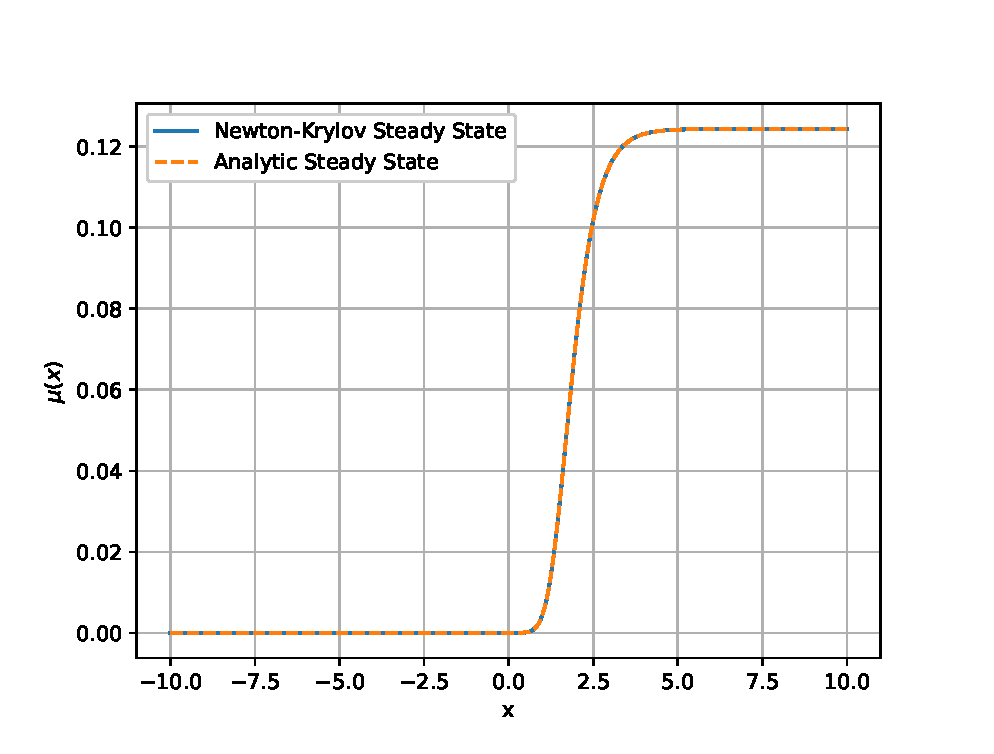
\includegraphics[width=\textwidth]{figures/nk_fp_chemotaxis_ss.eps}
    \end{subfigure}%
    \begin{subfigure}[b]{0.5\textwidth}
        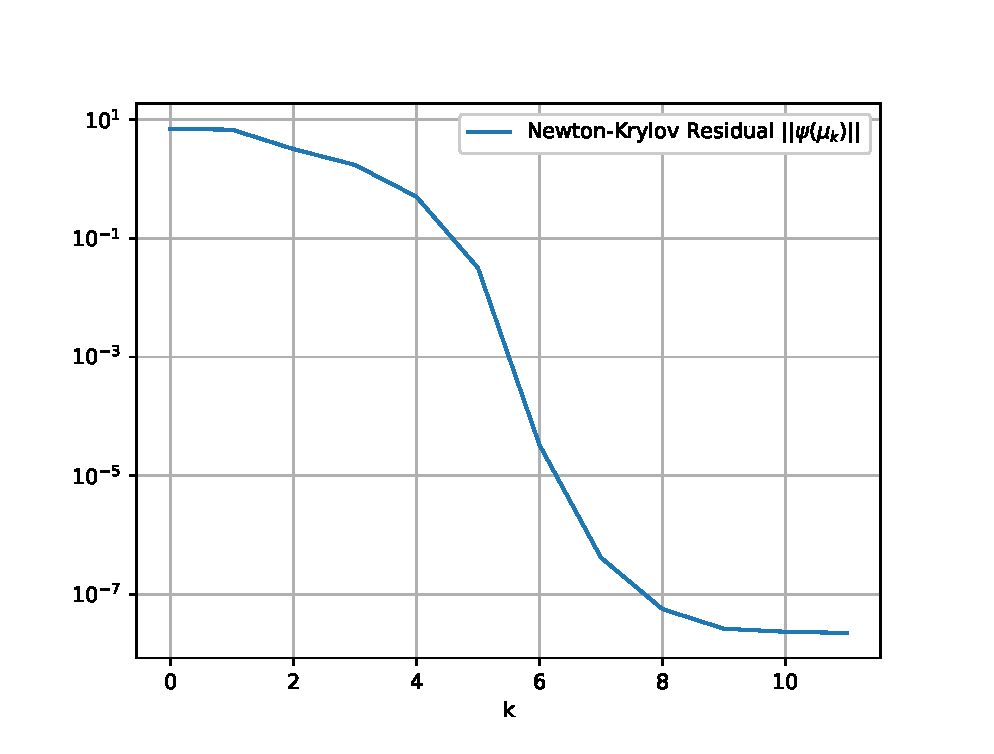
\includegraphics[width=\textwidth]{figures/nk_fp_chemotaxis_residual.eps}
    \end{subfigure}
    \caption{(Left) Steady-state distribution of the Keller-Segel model: Newton--Krylov (blue) vs. analytic solution (dashed orange). (Right) Newton-Krylov residual per iteration.}
    \label{fig:chemotaxis_fp}
\end{figure}

\begin{remark}
Even though the Fokker-Planck equation~\eqref{eq:keller-segel} and the $\Psi$-function are linear in $\mu_t$, the Newton-Krylov method is not guaranteed to converge to the steady-state distribution in one step, unlike the regular second-order Newton method. The reasons are twofold. First, the Newton-Krylov method does not solve the exact Jacobian system $D \psi(x_k) s_k + \psi(x_k) = 0$, rather an approximation $F(x_k, s_k) + \psi(x_k) = 0$. Secondly, we typically use a fixed tolerance $\eta_k = \eta > 0$ for all linear system solves. So instead of converging to the real steady-state distribution, the Newton-Krylov method will stay within a tolerance $\eta$ of the exact steady state, see also equation~\eqref{eq:backward_nk_error}.
\end{remark}

\subsubsection{Economic Agents Model} \label{subsusbec:agentmodel}
As a second demonstration of using Newton-Krylov to compute steady-state distributions of mean-field equations, let us consider the example of economic agents trading stocks. Each agent is represented by a value $X_i(t) \in (-1,1)$ that gives the tendency to buy ($X_i =1$) or sell ($X_i = -1$) a certain stock. More details on the model can be found here~\cite{fabiani2024task}. A McKean-Vlasov-type Euler timestepper for this model can be found on GitLab~\cite{} and we will use that timestepper in section~\ref{sec:w2_stochastics}. 

For this example, we look at the deterministic density $\mu(x,t)$ of the economic agents at location $x$ and time $t$. It can be shown that an approximate mean-field equation exists, of the form
\begin{equation} \label{eq:meanfield_agents}
    \partial_t \mu = \frac{1}{2} \sigma^2(t) \partial_{xx} \mu + \partial_x\left(b(x,t) \mu\right) + \left(J^+ + J^-\right) \delta(x).
\end{equation}
In this model, $b(x,t)$ and $\sigma^2(t)$ are the time-dependent drift and diffusivity of the agents, and $J^+$ and $J^-$ are integral operators with $\delta$ the Dirac-delta distribution. Further details on this model can be found in Appendix A of~\cite{fabiani2024task}. Importantly, this mean-field PDE is nonlinear, non-local and admits multiple steady-state distributions. 

\begin{figure}[!ht]
    \centering
    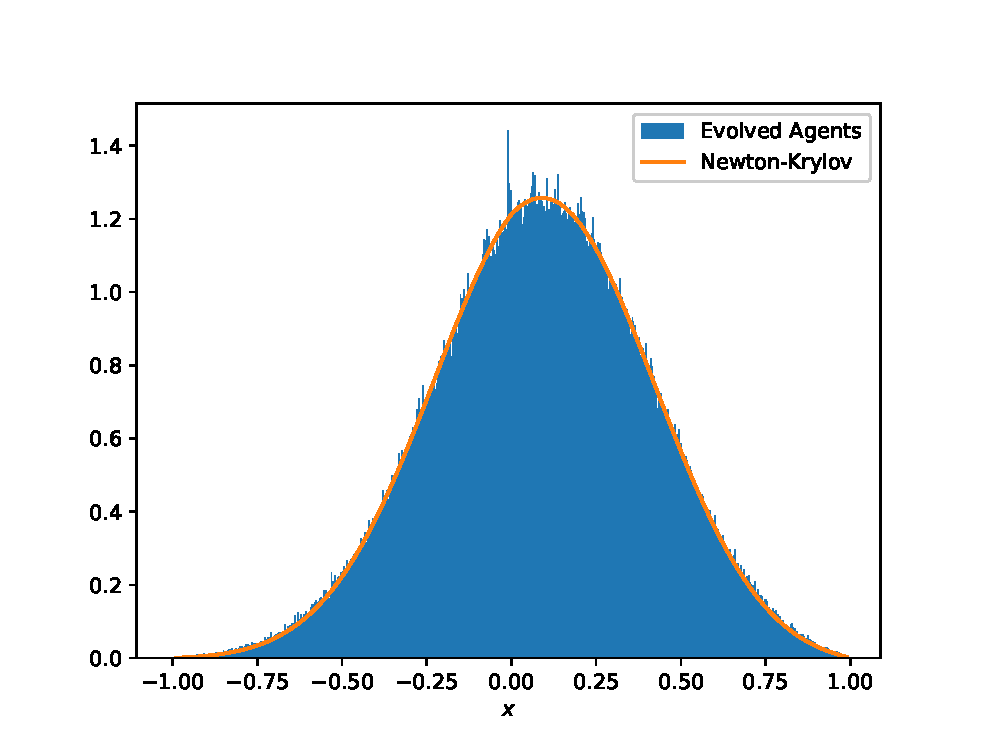
\includegraphics[width=0.7\textwidth]{figures/PDE_agents_ss.eps}
    \caption{Steady-state distribution from Newton--Krylov versus time evolution of stochastic agents.}
    \label{fig:agent_pde_ss}
\end{figure}

For the following numerical experiment, we discretized~\eqref{eq:meanfield_agents} using a finite-volume method with $N=100$ equidistant volume centers. Our PDE timestepper uses an explicit Euler method with step size $\Delta t = 10^{-4}$, and we integrate over a time window of size $1$ second. Figure~\ref{fig:agent_pde_ss} shows the steady-state distribution calculated by Newton-Krylov method in orange. It also shows the histogram distributions of the random agents obtained by timestepping the stochastic model to steady state. There is an excellent visual agreement between the two, as well as in the average agent position $\langle X_i \rangle$ of $0.0892$.

\section{Optimizers for Particle Timesteppers} \label{sec:w2_stochastics}
In this section we transition from deterministic PDE timesteppers to stochastic particle codes and the computation of their steady states. In the deterministic setting we wrote the fixed-point condition in residual form
\begin{equation}
\psi(x) = x-\phi_T(x) = 0
\end{equation}
and solved $\psi=0$ with Newton–Krylov. For particle timesteppers, however, a one-step map is inherently random, $y=\phi_T(x;\xi)$ where $\xi$ is the collection of random numbers used in propagating the particles. Even at equilibrium, individual particles keep moving due to the intrinsic noise $\xi$. An example is the random motion of molecules, even in thermal and statistical equilibrium. More generally, particles move at certain probabilities and `detailed balance' must be maintained in equilibrium. Hence the point-wise condition $\psi(x)=x-\phi_T(x)=0$ is not well defined. 

The steady state must be understood at the level of distributions: a distribution $\mu^\star$ is stationary when the distribution obtained after one step from $\mu^\star$ coincides with $\mu^\star$ again. However, distributions are not readily available from particle codes and must be built using histograms or tools like kernel density estimation. These methods for approximating the underlying distribution are sometimes and noisy as the particles themselves, and they are resource-intense to construct.

Instead, to cast this distributional steady state as an optimization problem, we work in Wasserstein geometry and measure the mismatch between the current distribution and its one-step image using the $2$-Wasserstein distance. Writing $X \sim \mu$ and $Y=\phi_T(X,\xi)$, the objective
\begin{equation}
    \mathcal{J}(\mu) = \tfrac12\,W_2^2\!\big(\mu,\ \text{law}(Y)\big)
\end{equation}
is nonnegative and vanishes if and only if $\mu$ is stationary. The Wasserstein distance directly ties into the heart of optimal transport theory and we will use some of those results here. In practice we represent $\mu$ by particles $X=\{x_i\}_{i=1}^N$ and, for a fixed noise seed $\xi$, form the one-step cloud $Y=\{y_i\}_{i=1}^N$. The sample objective
\begin{equation} \label{eq:discrete_W2}
    \mathcal{J}_N(X;\xi)= \tfrac12\,W_2^2\!\big(X, \phi_T(X,\xi))\big)
\end{equation}
becomes our optimization target over the initial particle locations $X$. Between changes of the optimal transport coupling, $\mathcal{J}_N$ is a smooth quadratic in the particle locations, and its (sub)gradient with respect to each $x_i$ is the transport displacement from $x_i$ to its match under the current optimal plan. This naturally leads us to first-order optimization methods to minimize~\eqref{eq:discrete_W2} such as (stochastic) gradient descent or Adam. We give more details on the Wasserstein formulation in section~\ref{subsec:wasserstein_formulation} and gradient-based optimization, with numerical results, in section~\ref{subsec:wasserstein_results}.

One might wish to recover the second-order performance of Newton–Krylov by solving
\begin{equation}
F(X)=\partial_X W_2^2\!\big(X,\ \phi_T(X)\big)=0
\end{equation}
and approximating Jacobian–vector products as
\begin{equation}
DF(X)\cdot v \approx  \frac{F(X+\varepsilon v)-F(X)}{\varepsilon}.
\end{equation}
In practice this is ill-posed and noisy for particle OT. The mapping $X\mapsto \partial_X W_2^2(X,\phi_T(X,\xi)$ is only piecewise smooth: as particles move, the optimal transport coupling changes combinatorially, creating kinks where $DF(X)$ does not exist. Difference quotients then mix values across distinct couplings, producing large, non-vanishing errors that blow up as $\varepsilon \to 0$. Stochasticity compounds the problem: tiny perturbations $X \mapsto X+\varepsilon v$ can reshuffle assignments in the empirical OT, injecting high-variance jumps into $F(X+\varepsilon v)-F(X)$. Krylov iterations driven by such JVPs become unstable, and line searches lose reliability. We perform a more detailed error analysis of the Newton-Krylov method for noisy objective functions in section~\ref{subsec:nk_noisy}, before moving on to using Newton-Krylov on smooth representations of particle codes in section~\ref{sec:particles_to_smooth}.

\subsection{Wasserstein distance formulation and optimization} \label{subsec:wasserstein_formulation}
We replace zeroing the ill-defined point-wise residual $\psi(X)=0$ by the Wasserstein distance in optimal-transport geometry. With $X=\{x_i\}{i=1}^N$ the current particle cloud and $Y=\phi_T(X;\xi)=\{y_j\}_{j=1}^N$ the one–step cloud for a fixed seed $\xi$, we minimize
\begin{equation} \label{eq:w2_objective}
F(X) = \tfrac{1}{2} W_2^2\big(X,Y\big)
 = \tfrac{1}{2}\min_{P\in\Pi}\ \sum_{i,j} P_{ij},|x_i-y_j|^2,
\end{equation}
where $\Pi$ is the optimal transport map between $X$ and $Y$, typically represented by a $N\times N$ doubly stochastic matrix (for distinct 1D points this is just a permutation~\cite{}). Let $\Pi^\star(X,Y)$ denote the optimal plan. The gradient of $F$ with respect to $X$ reads
\begin{equation} \label{eq:w2_gradient}
    \nabla F(X) = X - \Pi^\star Y + D\phi_T(X; \xi)\left(\phi_T(X,\xi) - (\Pi^\star)^{\top} X\right).
\end{equation}
In principle, we can evaluate this gradient and plug it into any first-order optimization algorithm, such as the Adam optimizer.

From a numerical point of view, the second term of~\eqref{eq:w2_gradient} poses a problem. Two subsequent evaluations of $F(X)$ for the same particles $X$ might differ due to the influence of $\xi$. In particular, this means that the Jacobian of the timestepper $D\phi_T(X; \xi)$ will be very noisy, even if we can evaluate it exactly through automatic differentiation. More importantly, this Jacobian will contain little actual information about the drift of the particles. Fortunately, by the Envelope theorem~\cite{}, we can use only the first term of the gradient
\begin{equation}
\partial_X \tfrac{1}{2}W_2^2(X,Y) = X - \Pi^\star Y
\end{equation}
for optimization purposes. This (partial) gradient is much better conditioned and numerically more stable.

There remains one more computational bottleneck in this Wasserstein-minimization algorithm, and that is the computation of the optimal transport map $\Pi^\star$. In one dimension, sorting both clouds and matching in order yields $\Pi^\star$ in $\mathcal{O}(N\log N)$ time. This is the theoretically optimal complexity. In multiple dimensions, one may use a linear assignment solver which is typically very expensive, i.e., $\mathcal{O}(N^3)$ . We will showcase the Wasserstein-minimization approach on both one- and two-dimensional examples in the next section.

For any initial set of particles $X$, we can evaluate $F(X)$ and its gradient $\partial_X F(X)$. We can therefore minimize $F$ with any first-order scheme; we use Adam because of its stability under mild noise. A typical iteration is as follows
\begin{enumerate}
\item Given $X_k$ and random numbers $\xi_k$, compute $Y_k=\phi_T(X_k;\xi_k)$.
\item Compute an optimal plan $P_k^\star=P^\star(X_k,Y_k)$.
\item Form the gradient $g_k=X_k-P_k^\star Y_k$ (optionally average over a small batch of independent runs for variance reduction).
\item Apply Adam to obtain $X_{k+1}$.
\end{enumerate}
We use PyTorch's Adam optimizer in our implementation. One advantage of PyTorch is that we can use its call graph to directly compute gradients of $F(X)$. The first term of that gradient can then be obtained by detaching $Y$ from the call graph.

In summary, minimizing $F(X)=\tfrac12 W_2^2(X,\phi_T(X;\xi))$ with Adam yields a fast $\mathcal{O}(N \log N)$ procedure that is robust to stochasticity and faithful to the Wasserstein fixed-point formulation, while avoiding the instability of second-order information at coupling changes.

\subsection{Three Examples} \label{subsec:wasserstein_results}
The Wasserstein-gradient flow is a well-defined, easy-to-implement, and reliable approach to compute steady-state distributions of particle methods. Combining gradient flow with the Adam optimizer also has significant advantages such as steady decrease of the $W_2^2$-loss. In this section, we demonstrate the combined method on three examples: bacterial chemotaxis (section~\ref{subsubsec:w2_chemotaxis}), the nonlinear economic agents model (section~\ref{subsubsec:w2_agents}), and a two-dimensional overdamped Langevin dynamics with non-trivial potential energy profile (section~\ref{subsubsec:w2_halfmoon}).

\subsubsection{Bacterial Chemotaxis} \label{subsubsec:w2_chemotaxis}
We discretize the overdamped Langevin dynamics in equation~\eqref{eq:chemotaxis} using an Euler-Maruyama method with step size $\Delta t = 10^{-3}$, and per evaluation of the timestepper $\phi_T(\cdot)$ we integrate up to $T = 1$ seconds. Reflective boundary conditions are applied after every Euler-Maruyama step. We run the Adam optimizer with standard parameters ($\beta_1 = 0.9, \beta_2=0.99$) and an initial `learning rate' of $10^{-1}$. We decrease the learning rate by a factor $10$ every $100$ epochs, for a total of $300$ epochs. The initial distribution is a truncated Gaussian with a mean $5$ and a standard deviation of $2$.

As we see in Figure~\ref{fig:w2_chemotaxis}, the Wasserstein-Adam optimizer reliably converges to a final loss of $2 \ 10^{-5}$. The loss gradient also decreased to a similar value, indicating strong convergence. The histogram of the optimized particles (right figure, orange) also matches well with the analytic invariant distribution. Finally, we see in the figure on the left that the Wasserstein-Adam optimizer reached this steady-state already after about $150$ epochs - or a total simulation time of $150$ seconds. This is because the objective function is evaluated only once per Adam epoch. Compared to computing the steady-state by long-time evolution of~\eqref{eq:chemotaxis}, which takes about $500$ seconds of in-simulation time, the Wasserstein-Adam method is much faster.

\begin{figure}[h]
    \centering
    \begin{subfigure}[b]{0.51\textwidth}
        \centering
        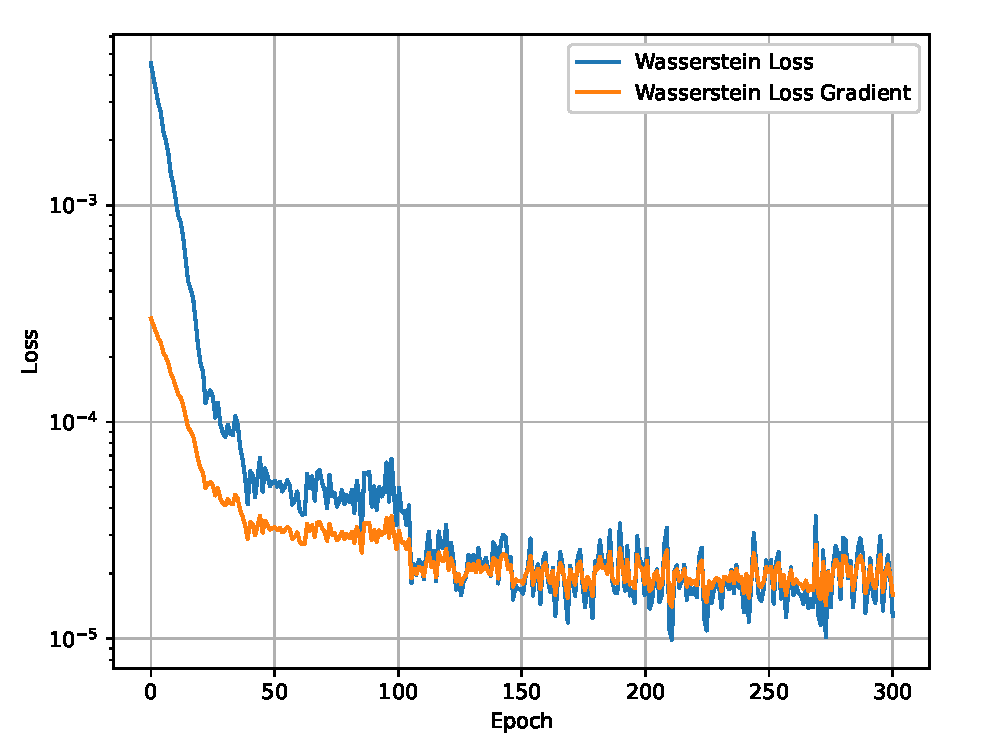
\includegraphics[width=\textwidth]{figures/WassersteinChemotaxisLoss.eps}
    \end{subfigure}%
    \begin{subfigure}[b]{0.51\textwidth}
        \centering
        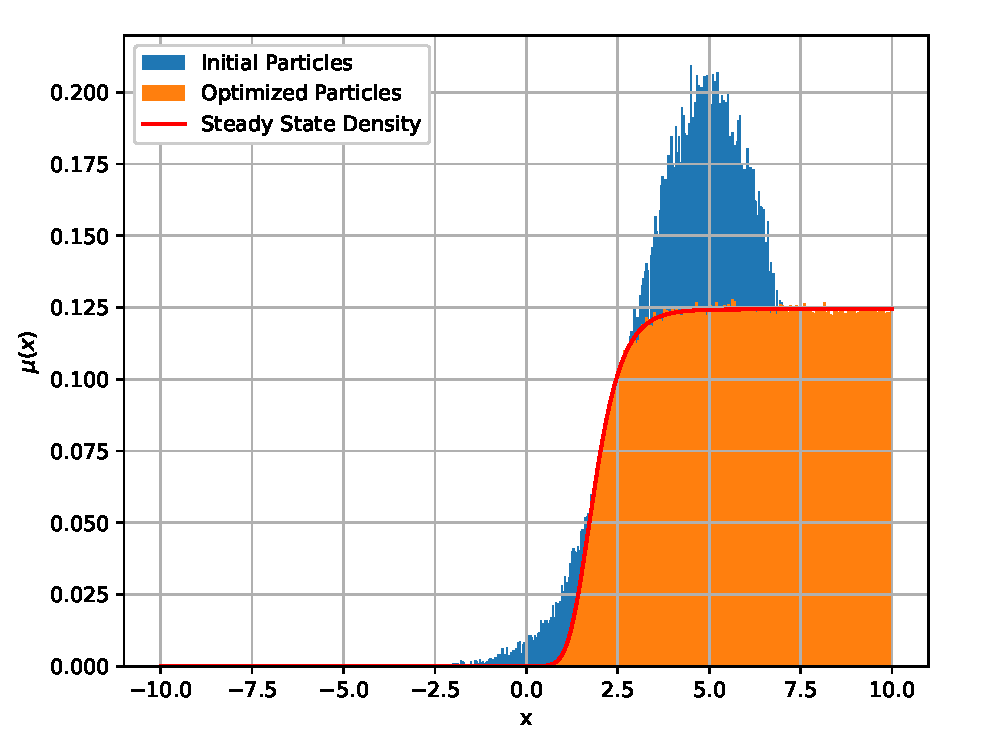
\includegraphics[width=\textwidth]{figures/WassersteinChemotaxisParticles.eps}
    \end{subfigure}
    \caption{Numerical results for the Wasserstein-Adam optimizer on the chemotaxis model. Left: Wasserstein loss (blue) and gradient-norm (orange) per epoch. Right: Histogram of the initial particles in blue, the Wasserstein-Adam optimized particles in orange, and the analytic steady-state density (see equation~\eqref{eq:chemotaxis_ss}) in red.}
    \label{fig:w2_chemotaxis}
\end{figure}

\subsubsection{Economic Agents} \label{subsubsec:w2_agents}
The Wasserstein-Adam method also works well for nonlinear models such as the economic agents model from section~\ref{subsusbec:agentmodel}. We use the timestepper available at~\cite{} to integrate the agents up to $T = 1$ seconds at a time. This timestepper is unbiased for the dynamics of the agents' dynamics and uses the discretization presented in~\cite{}. We again use an Adam optimizer with an initial learning rate of $10^{-1}$ and with standard parameters to find the steady-state distribution of the particles. The learning rate is decreased by a factor $10$ every $100$ epochs for a total of $300$ epochs. The initial distribution is a Gaussian with zero mean and a standard deviation of $0.1$. The steady-state distribution is wider and approximately normal.

Figure~\ref{fig:w2_agents} displays the Wasserstein loss and gradient on the left, as well as optimized agents compared to the steady-state distribution on the right. The initial distribution of agents is shown too. We observe an excellent match between the histogram of optimized agents and the invariant distribution. The loss stagnates near $2 \ 10^{-6}$, nearly four orders of magnitude lower than the initial loss, demonstrating a clear convergence.

\begin{figure}[h]
    \centering
    \begin{subfigure}[b]{0.51\textwidth}
        \centering
        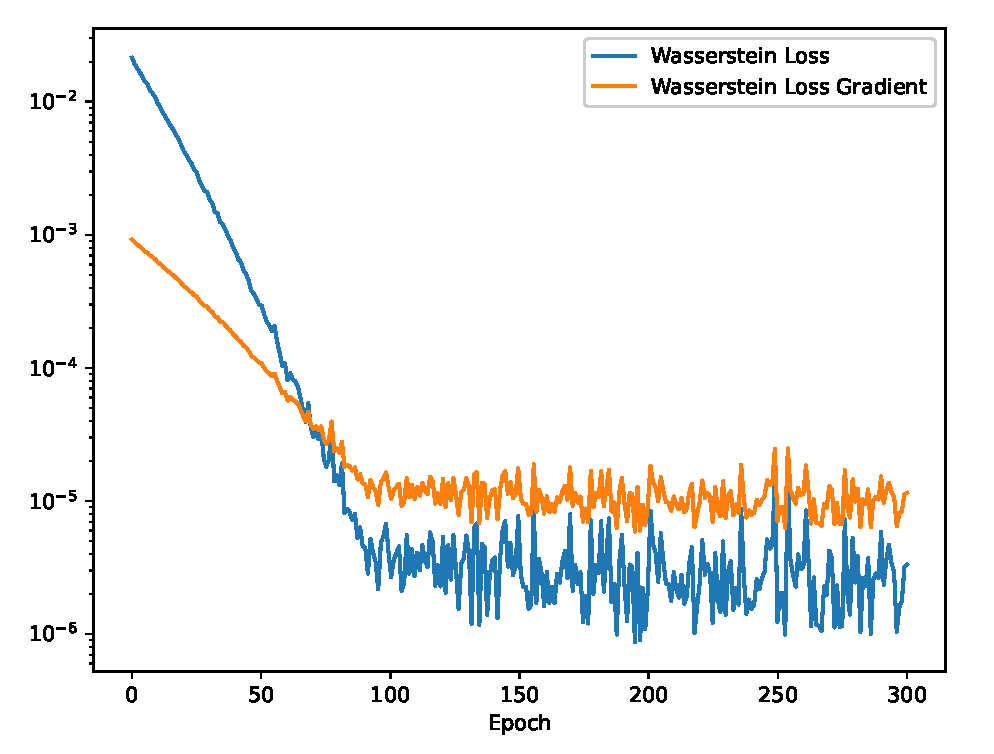
\includegraphics[width=\textwidth]{figures/WassersteinAgentsLoss.eps}
    \end{subfigure}%
    \begin{subfigure}[b]{0.51\textwidth}
        \centering
        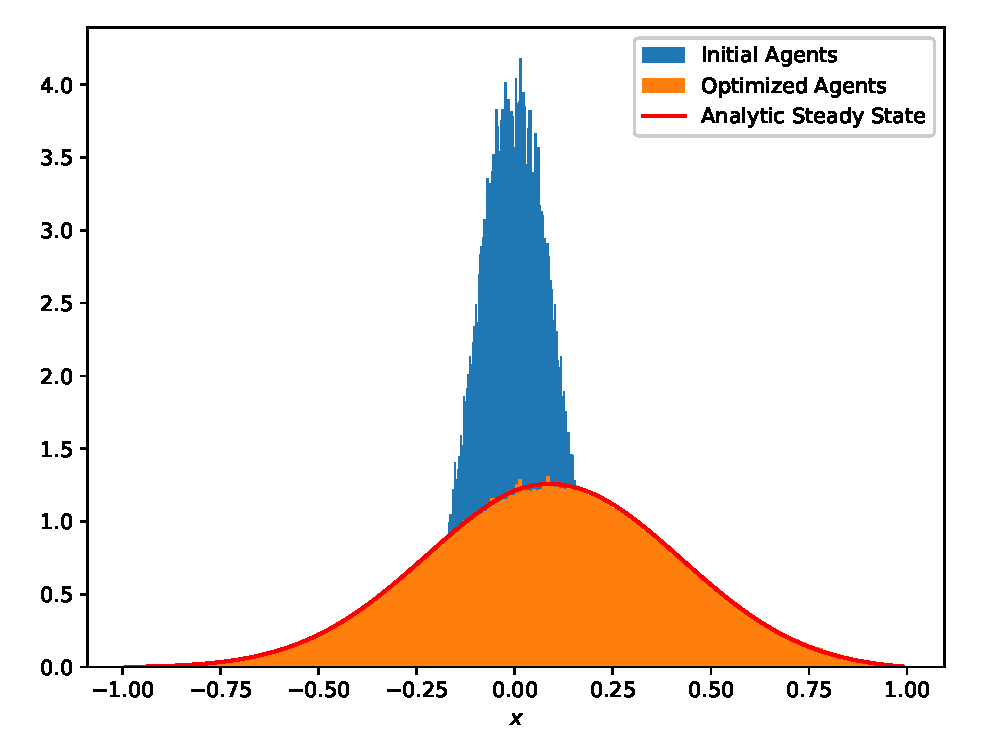
\includegraphics[width=\textwidth]{figures/WassersteinAgentsParticles.eps}
    \end{subfigure}
    \caption{Numerical results for the Wasserstein-Adam optimizer on the economic agents model. Left: Wasserstein loss (blue) and gradient-norm (orange) per epoch. Right: Histogram of the initial particles in blue, the Wasserstein-Adam optimized particles in orange, and the analytic steady-state density (see Figure~\ref{fig:agent_pde_ss}) in red.}
    \label{fig:w2_agents}
\end{figure}

\subsubsection{The Half-Moon Potential} \label{subsubsec:w2_halfmoon}
In multiple dimensions one cannot exploit the monotone rearrangement used in 1D (sorting), so computing $W_2$ requires solving a discrete assignment problem between the two point clouds. We use the Hungarian solver, whose worst-case complexity is $\mathcal{O}(M^3)$ for $M$ paired points; applied to the full cloud this would be $\mathcal{O}(N^3)$. To keep costs manageable, we adopt mini-batches of size $B$: each step solves an $\mathcal{O}(B^3)$ assignment and we process $N/B$ batches per iteration, yielding a total $\mathcal{O}(NB^2)$ complexity. The smaller the batch size, the smaller the computational cost. The rest of the Wasserstein–Adam flow is unchanged from 1D: we form $Y_b=\varphi_T(X_b)$, compute an optimal matching $\Pi_b^\star$ on each batch $b$, use the detached gradient $\partial_X \tfrac{1}{2} W_2^2(X_b, Y_b) = X_b-\Pi_b^\star Y_b$, and update the particles $X_b$ with Adam.

For this example, we consider a two-dimensional half-moon potential. The potential energy function $U(x,y)$ is given by
\begin{equation} \label{eq:halfmoonpotential}
    U(x, y) = A \left(r(x,y) - R\right)^2 + B \exp\left( - \alpha (y - y_s)\right)
\end{equation}
with $A = 2, B= 0.5, R = 2, \alpha=1.5$, and $y_s=-0.5$. The function $r(x,y) = \sqrt{x^2+y^2}$ measures the distance from the origin. A two-dimensional color plot of the corresponding steady-state distribution
\begin{equation} \label{eq:halfmoon_dist}
    \mu(x,y) = Z^{-1} \exp\left(-U(x,y)\right)
\end{equation}
is shown in Figure~\ref{fig:halfmoonpotential}.

\begin{figure}
    \centering
    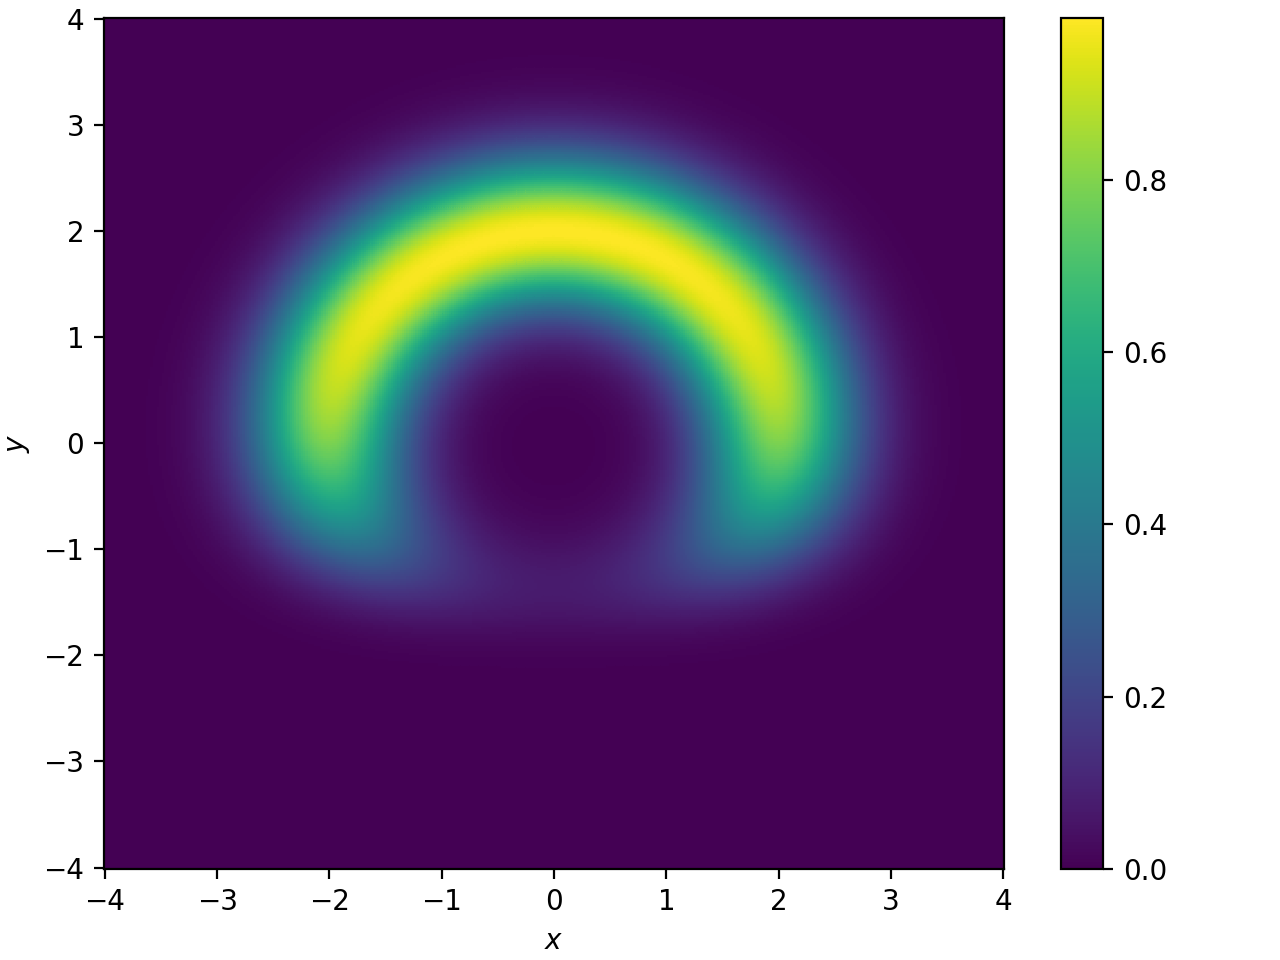
\includegraphics[width=0.8\linewidth]{figures/HalfMoon.png}
    \caption{A color plot of the half-moon potential, see equation~\eqref{eq:halfmoonpotential} for more details.}
    \label{fig:halfmoonpotential}
\end{figure}

To compute the steady-state distribution using the Wasserstein-Adam method, we construct an overdamped Langevin dynamics of the form
\begin{equation} \label{eq:langevin_halfmoon}
    d(X,Y) = -\nabla U(X,Y) dt + \sqrt{2} dW_t
\end{equation}
where $W_t$ is a two-dimensional Brownian motion with independent components. The steady-state distribution of this dynamics is precisely~\eqref{eq:halfmoon_dist}. We also implement reflective boundary conditions (e.g., Neumann) to keep all particles within the domain $[-4,4] \times [-4,4]$. We discretize this overdamped Langevin dynamics using the Euler-Maruyama timestepper with step size $\Delta t = 10^{-3}$, and integrate up to time $T = 0.1$ seconds. The initial distribution is a standard bivariate Gaussian, which has minimal overlap with~\eqref{eq:halfmoon_dist}.

To compute the Wasserstein loss, we divide the $N=10^5$ particles into batches of size $1000$. For each batch, we propagate the particles through the timestepper and evaluate the loss using the Hungarian algorithm. We feed these batches to the Adam optimizer, which uses an initial learning rate of $10^{-2}$, decreasing by a factor of $10$ every $100$ epochs, up to $300$ epochs. 

The optimization results are shown in Figure~\ref{fig:w2_halfmoon}. The left panel reports the objective and gradient-norm trajectories: the initial $\tfrac12 W_2^2$ of $0.51233$ decreases monotonically to $1.54\times10^{-2}$, effectively reaching the stochastic noise floor, and the loss gradient decays in tandem, indicating stable convergence. The right panel displays a 2D histogram (colormap) of the optimized particles, which shows an excellent match to the analytic steady-state distribution from figure~\ref{fig:halfmoonpotential} with no visible systematic bias.

\begin{figure}[h]
    \centering
    \begin{subfigure}[b]{0.51\textwidth}
        \centering
        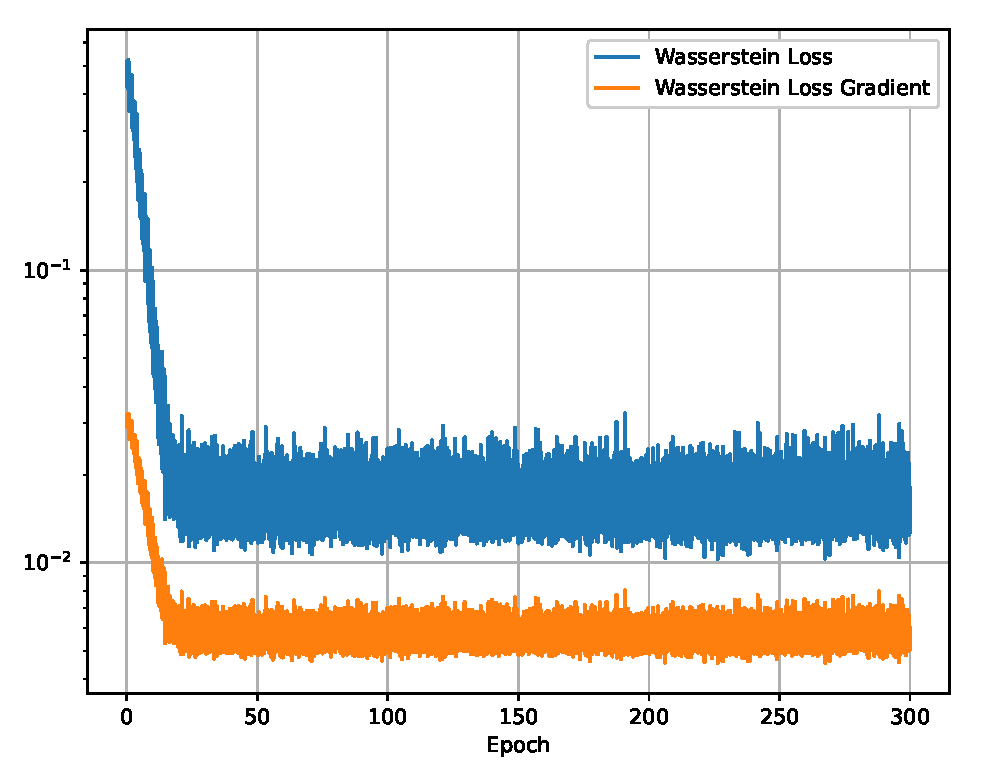
\includegraphics[width=\textwidth]{figures/WassersteinHalfMoonLoss.eps}
    \end{subfigure}%
    \begin{subfigure}[b]{0.51\textwidth}
        \centering
        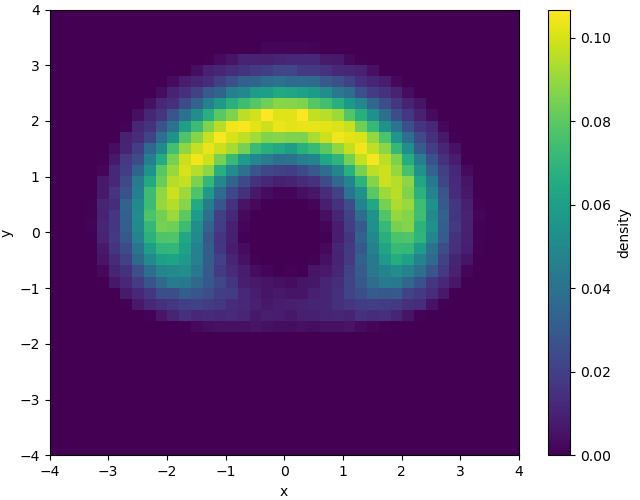
\includegraphics[width=\textwidth]{figures/WassersteinHalfMoonHistogram.png}
    \end{subfigure}
    \caption{Numerical results for the Wasserstein-Adam optimizer on the half-moon potential. Left: Wasserstein loss (blue) and gradient-norm (orange) per epoch. Right: Colormap of the 2D histogram of the optimized particles in orange.}
    \label{fig:w2_halfmoon}
\end{figure}

\subsection{Extending the Error Analysis to Stochastic Timesteppers} \label{subsec:nk_noisy}
We aim for faster convergence to steady state than is attainable with first-order Wasserstein gradient flow through gradient-based optimizers. A natural idea is to invoke second-order optimization, yet in the particle setting the underlying derivatives are not fully well defined [\textbf{Need some theory here}]. The basic idea would be to start from the Wasserstein objective function~\eqref{eq:w2_objective} and solve for a zero (truncated) gradient 
\begin{equation} \label{eq:nk_particle_objective}
    G(X) = \partial_X \tfrac{1}{2} W_2^2\left(X, \phi_T(X)\right) = X - \Pi^\star \phi_T(X),
\end{equation}
where $\Pi^\star$ is the optimal transport map from $X$ to $Y = \phi_T(X)$. For any finite number of particles $N$ there will be a noise term for each evaluation of the Wasserstein objective function. Indeed,
\begin{equation}
    \tfrac{1}{2} W_2^2(X, \phi_T(X)) = \tfrac{1}{2}W_2^2(\mu, \text{law}(Y)) + \frac{\xi}{\sqrt{N}},
\end{equation}
where $\mu$ is the distribution of samples $X$. We do not assume anything about the distribution of the noise term $\xi \in \mathbb{R}$ -- only that it is independent of $X$. The gradient objective function~\eqref{eq:nk_particle_objective} will then also include a noise term
\begin{equation} \label{eq:nk_particle_objective_noise}
    \tilde{G}(X) = G(X) + \frac{\zeta}{\sqrt{N}}
\end{equation}
where the contributions per-component of $\zeta \in \mathbb{R}^N$ add up to $\xi$.

Any second-order optimization method will require Jacobians of the objective function in equation~\eqref{eq:nk_particle_objective}. In the Newton-Krylov method, the action Jacobian of $G$ in the direction of $v$ is approximated by finite differences. Under the assumption that subsequent evaluations of $G$ introduce independent noise terms $\zeta_1$ and $\zeta_2$, approximating the action of the Jacobian $D G$ on a vector $v$ introduces an additional variance term that scales unfavorably as the step size $\varepsilon \to 0$
\begin{equation} \label{eq:nk_particles_Gv}
D \tilde{G}(X)v \approx \frac{\tilde{G}(X+\varepsilon v) - \tilde{G}(X)}{\varepsilon} = \frac{G(X+\varepsilon v) - G(X)}{\varepsilon} + \frac{\zeta_1 - \zeta_2}{\varepsilon\sqrt{N}}.
\end{equation}
Since $\zeta_1$ and $\zeta_2$ are independent, for example, through independent random numbers in the timestepper, and $\varepsilon$ is typically small (say $\sqrt{\varepsilon_{\text{mach}}} \approx 10^{-8}$), the resulting noise term $(\zeta_1 - \zeta_2) / \varepsilon\sqrt{N}$ will dominate the Jacobian-vector product. The estimated Jacobian therefore carries essentially no usable descent information, and the Newton–Krylov method will degenerate into stochastic oscillations rather than a systematic search direction, failing to converge toward the true steady state. Continuing the error analysis from Section~\ref{sec:nk}, the asymptotic error of the Newton-Krylov method is governed by a fundamental bias–variance trade-off,
\begin{equation} \label{eq:nk_particle_error}
\norm{X_\infty - X^\star} \leq C\norm{G(X^\star)^{-1}}\left( \varepsilon + \limsup_{k} |\eta_k| + \varepsilon_{\text{mach}} + \frac{2\sigma}{\varepsilon \sqrt{N}} \right)
\end{equation}
where $\sigma$ is the standard deviation of $\xi$. The above equation highlights the challenge of second-order methods on the level of particles: although they carry the potential for rapid convergence, the noise inherent in particle-based Jacobians fundamentally limits their accuracy. However, we can use equation~\eqref{eq:nk_particle_error} to determine $\varepsilon$ so that the approximation and noise terms are balanced. It can be seen that the minimal total error is achieved when $\varepsilon = \mathcal{O}\left(N^{-1/4}\right)$. As an example, for $N=10^4$, we would need to use $\varepsilon = 0.1$ -- which is much larger than $\sqrt{\varepsilon_{\text{mach}}}$ in the absence of noise.

However, even with this optimal finite-difference step size, Newton-Krylov at the particle level cannot discern any gradient information from~\eqref{eq:nk_particles_Gv}. Let us consider the bacterial chemotaxis example again from section~\ref{subsubsec:w2_chemotaxis}. In Figure~\ref{fig:nk_particles_chemotaxis} we show the Newton-Krylov optimization result after $100$ steps with $N=10^5$ particles and $\varepsilon = 0.1$. The optimized particles barely moved from their initial distribution. Figure~\ref{fig:nk_particles_chemotaxis} shows the norm of the objective function~\eqref{eq:nk_particle_objective_noise} in all iterations, revealing that the error remains essentially unchanged in expectation. The reason for this behavior is that although each application of the timestepper moves the particles closer to the steady state, the subsequent Newton–Krylov update perturbs them in essentially random directions. As a result, the timestepper is forced to repeatedly recover the same progress, preventing any net convergence.

\begin{figure}[h]
    \centering
    \begin{subfigure}[b]{0.51\textwidth}
        \centering
        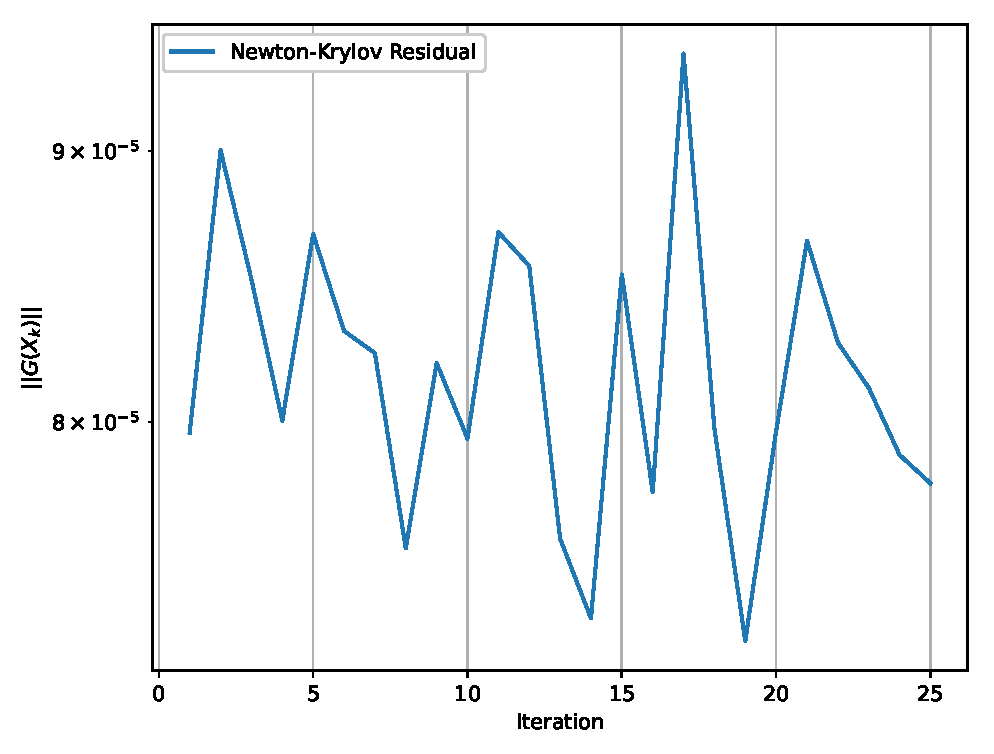
\includegraphics[width=\textwidth]{figures/NK_Chemotaxis_Loss.eps}
    \end{subfigure}%
    \begin{subfigure}[b]{0.51\textwidth}
        \centering
        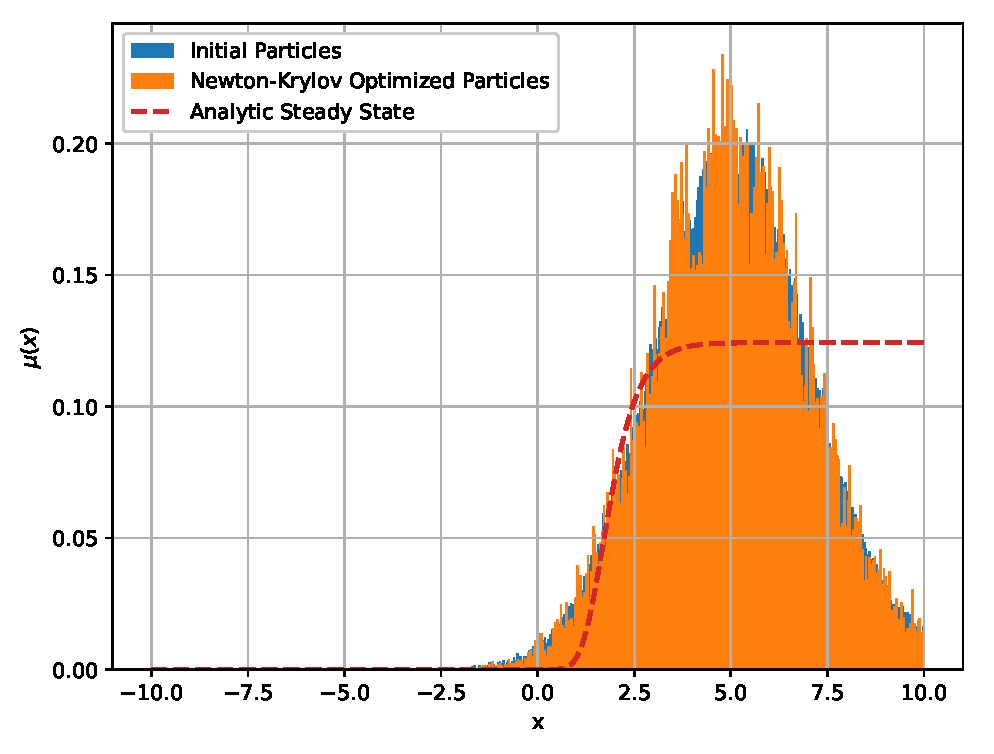
\includegraphics[width=\textwidth]{figures/NK_Chemotaxis_particles.eps}
    \end{subfigure}
    \caption{Numerical results for the Newton-Krylov optimizer for bacterial chemotaxis. Left: Norm of the objective function, $\norm{\tilde{G}(X_k)}$ per iteration. Right: Initial particles (blue), optimized particles (orange) and analytic steady-state distribution (dashed red).}
    \label{fig:nk_particles_chemotaxis}
\end{figure}

\section{From Particles to Smooth Representations} \label{sec:particles_to_smooth}
Newton–Krylov may not work on the level of noisy particles, but it can work if we add smoothness to the optimization criterion. Enter the inverse cumulative density function. In one dimension, optimal transport with respect to the Wasserstein-2 distance admits an especially convenient formulation. Composing the ICDF with the CDF of the particles is exactly equivalent to computing the optimal transport map, ensuring that the geometry of the problem is preserved. Furthermore, the inverse cumulative density function (ICDF) provides a smooth, monotonic representation of the empirical measure. The ICDF is continuously differentiable, so we can employ Newton-type methods to calculate steady states. Finally, evaluating the ICDF at prescribed percentiles corresponds to drawing samples from the distribution.

These combined elements make it possible to define a timestepper directly at the level of the ICDF. Starting from the current ICDF, we first sample $N$ particles by evaluating the ICDF in the (fixed) $k/N$ percentiles. Next, we propagate these samples through the stochastic particle timestepper, after which we construct the new ICDF by retaining some of the (sorted) particles. In this representation, derivatives are well defined, and Newton-Krylov iterations can be applied meaningfully, recovering the fast convergence that is lost in the purely particle-based formulation.

Extending this idea beyond one dimension requires additional care. A global ICDF does not exist in higher dimensions, nor does the notion of a percentile. One must construct alternative smooth representations that retain the essential link to optimal transport theory. An option is to work with the two-dimensional cumulative distribution function (CDF), which generalizes the one-dimensional case and retains links to optimal transport. An alternative is the sliced Wasserstein distance. By projecting the distribution onto many one-dimensional directions, each projection yields an ICDF that is well defined, and these are aggregated to approximate the full Wasserstein geometry. Therefore, both the CDF and the sliced Wasserstein framework act as higher-dimensional analogues of the one-dimensional ICDF, providing the smoothness needed to construct well-behaved timesteppers and to restore the accelerated convergence of Newton–Krylov methods in the multidimensional setting.

\subsection{The ICDF-to-ICDF Timestepper}
Given a one-dimensional probability density $\mu(x)$ on a fixed interval $[a,b]$, the cumulative density function is defined as
\begin{equation} \label{eq:1d_cdf}
 F(x) = \int_{a}^x \mu(y)dy, \ \ x \in [a,b]
\end{equation}
Because $F$ is monotonic, it is injective and inverse cumulative density $F^{-1}(p)$ exists. This ICDF is defined for $p \in [0,1]$ and $x = F^{-1}(p)$ corresponds to the $p$-th percentile of $\mu$.

For a discrete set of (sorted) particles $\{X_n\}_{n=1}^N$, the cumulative density function is piecewise continuous with jumps at the locations
\begin{equation}
 F(X_n) = \frac{n}{N}.
\end{equation}
The inverse cumulative density function is also piecewise continuous defined in the discrete percentiles $F^{-1}\left(n/N\right) = X_n$. To reduce the impact of precise particle locations $X_n$, we propose to evaluate the ICDF in a fixed percentile grid $p_k, k=1,\dots,K$ - typically uniform between $0$ and $1$ - with $K \ll N$. This allows us to construct a coarse ICDF-to-ICDF timestepper
\begin{equation}
    \Phi_T\left(F^{-1}_t\right) = F^{-1}_{t+T}
\end{equation}
in four stages:
\begin{itemize}
    \item[1.] Interpolate $F^{-1}(t)$ on the fixed grid $p_k, k=1,\dots,K$ using a differentiable spline;
    \item[2.] Sample $\{X_n(t)\}$ by evaluating $F^{-1}(t)$ in uniform percentiles $n/N$;
    \item[3.] Propagate the particles to $\{X_n(t+T)\}$ using the particle timestepper $\phi_T$;
    \item[4.] Construct the new ICDF by sorting $\{X_n(t+T)\}$ and retaining every $K$-th particle.
\end{itemize}
A schematic of the ICDF-to-ICDF timestepper is shown in Figure~\ref{fig:icdftoicdf}.

\begin{figure}[!ht]
  \centering
  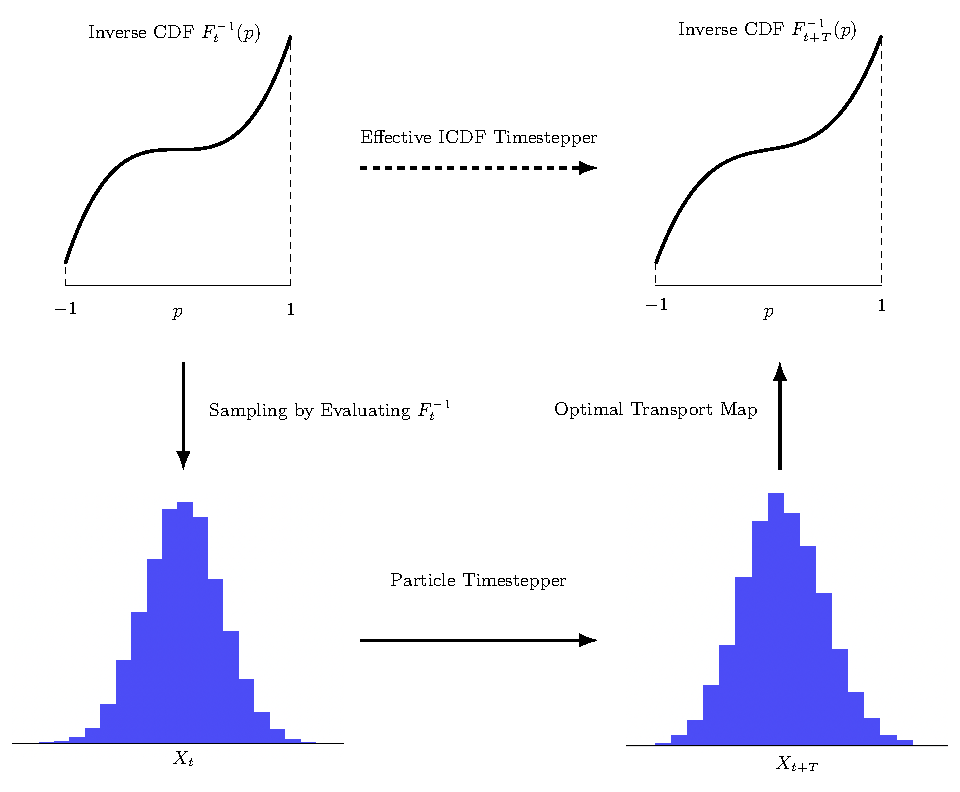
\includegraphics[width=0.8\textwidth]{ICDFtoICDF.pdf}
  \caption{Schematic of the effective ICDF–to-ICDF timestepper.}
  \label{fig:icdftoicdf}
\end{figure}

By construction, both the ICDF representation and its spline approximation ensure that the timestepper maps one smooth ICDF into another. In this setting, finite-difference approximations of the directional derivative $D\Phi_T \cdot v$ no longer suffer from variance-amplifying $1/\varepsilon$ terms, since the noise inherent at the particle level has been averaged out by the smooth representation. As a result, Newton–Krylov iterations regain their expected fast convergence toward the steady-state distribution, now expressed consistently through the ICDF. The associated ICDF-based objective function is given by
\begin{equation} \label{eq:icdf_residual}
\Psi(F^{-1}) = F^{-1}- \Phi_T(F^{-1}).
\end{equation}
which is zero in steady state. Notice that the error bound in equation~\eqref{eq:nk_particle_error} remains applicable, since the ICDF-to-ICDF timestepper is ultimately constructed from the underlying particle timestepper~$\phi_T$. However, because the ICDF provides a smooth aggregate representation of the ensemble, the effective noise variance~$\sigma^2$ is substantially reduced. As a result, the stochastic error in the finite-difference approximation becomes small enough for the method to operate within the stable, “workable” Newton–Krylov regime, where second-order convergence is dominant.

\subsection{Three Numerical Results}
We now demonstrate the performance of the Newton–Krylov method on the ICDF-to-ICDF timestepper through three examples. These examples illustrate the accuracy, robustness, and noise tolerance of Newton-Krylov on smooth particle representations across increasingly complex systems.

\subsubsection{The Bimodal Distribution Revisited}
As a first demonstration of the Newton–Krylov method applied to the ICDF-to-ICDF timestepper, we reconsider the bimodal distribution introduced in section~\ref{sec:trajectories}. The unknowns in this formulation are the values of the ICDF on a fixed percentile grid $p_k = (k - 0.5)/100$ for $1 \leq k \leq 100$. During each evaluation of the timestepper, we interpolate the ICDF using piecewise linear functions, sample $N = 10^5$ particles at equidistant percentiles, propagate them forward using the microscopic timestepper~$\phi_T$ over a time window of length~$T = 0.1$, and reconstruct the new ICDF by retaining every $1000$th particle (i.e. $N / 100$) in sorted order (i.e. after applying the optimal transport map). These retained particle locations define the updated ICDF on the fixed percentile grid at time~$T$. Jacobian–vector products are approximated by finite differences with a step size of~$\varepsilon = 10^{-2}$.

\begin{figure}[h]
    \centering
    \begin{subfigure}[b]{0.51\textwidth}
        \centering
        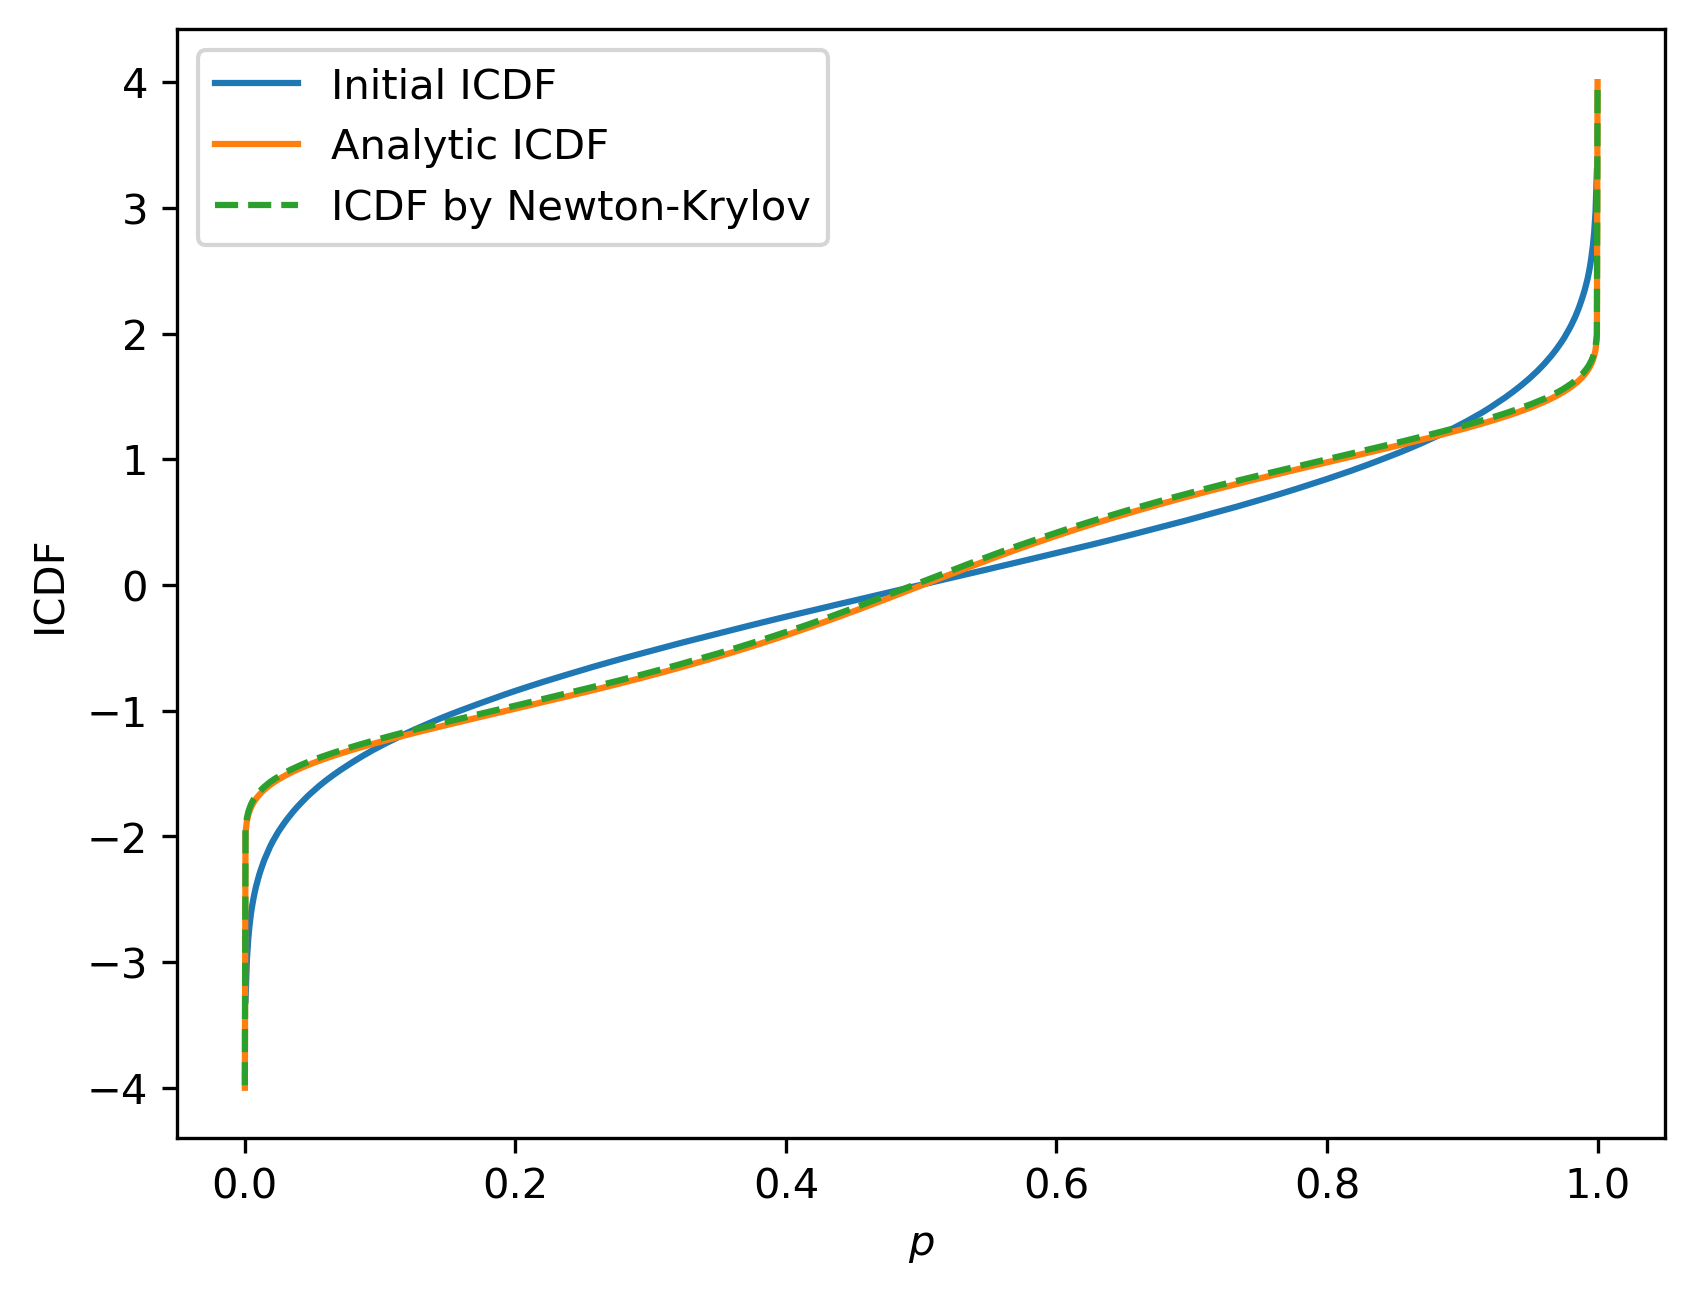
\includegraphics[width=\textwidth]{figures/BimodalICDF.png}
    \end{subfigure}%
    \begin{subfigure}[b]{0.51\textwidth}
        \centering
        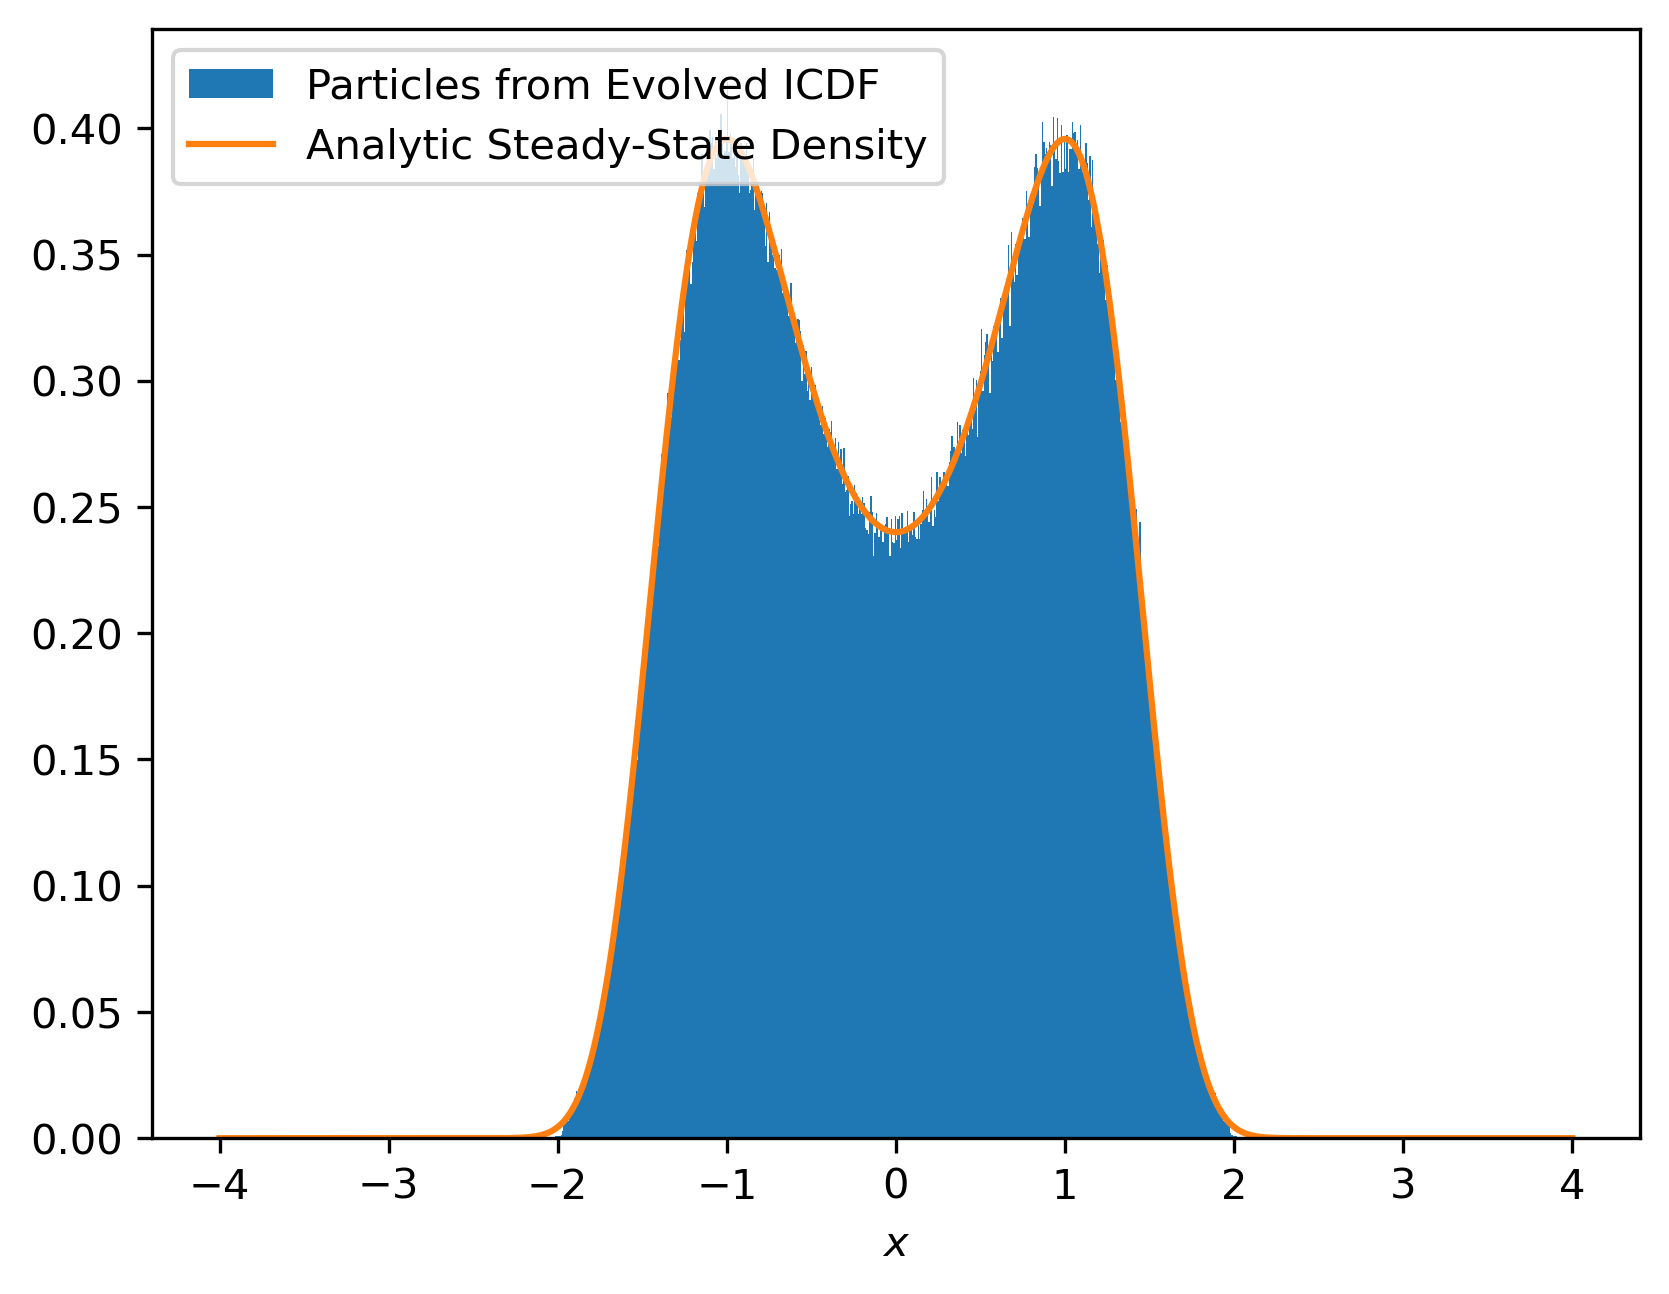
\includegraphics[width=\textwidth]{figures/ParticlesBimodalICDF.png}
    \end{subfigure}
    \caption{(Left) Initial (orange) true steady-state (blue) and steady-state ICDF computed by Newton-Krylov (dashed green). (Right) Particles sampled from the Newton-Krylov ICDF (blue) and corresponding steady-state bimodal density.}
    \label{fig:bimodal_icdf}
\end{figure}

The convergence behavior of Newton–Krylov on the ICDF timestepper is shown in Figure~\ref{fig:bimodal_icdf}. The left panel compares the ICDF of the initial guess—corresponding to a standard Gaussian—with the steady-state ICDF obtained after convergence. The right panel displays the histogram of $N = 10^5$ particles sampled from this steady-state ICDF, showing excellent agreement with the analytical bimodal invariant distribution. For completeness, we also report the residual norm $\norm{\Psi\left((F^{-1})^{(k)}\right)}$ per Newton–Krylov iteration~$k$, which decreases rapidly to a noise floor around $10^{-2}$. This residual level is consistent with the theoretical prediction from equation~\eqref{eq:nk_particle_error}.

\subsubsection{Bacterial Chemotaxis}
As a second example, we revisit the bacterial chemotaxis model introduced in section~\ref{subsubsec:w2_chemotaxis}. The ICDF is again discretized on a fixed percentile grid $p_k = (k - 0.5)/100$, for $1 \leq k \leq 100$. At each timestepper evaluation, we interpolate the ICDF using piecewise linear functions, sample $N = 10^5$ particles at equidistant percentiles, and propagate them over a time horizon of $T = 1$ second using the microscopic particle timestepper described in section~\ref{subsubsec:w2_chemotaxis}. The propagated ensemble is then projected back onto the ICDF representation by sorting the particle locations. The initial distribution is again taken to be a Gaussian with mean $5$ and standard deviation $2$, and Jacobian–vector products are again evaluated using finite differences with step size $\varepsilon = 10^{-1}$.

\begin{figure}[h]
    \centering
    \begin{subfigure}[b]{0.51\textwidth}
        \centering
        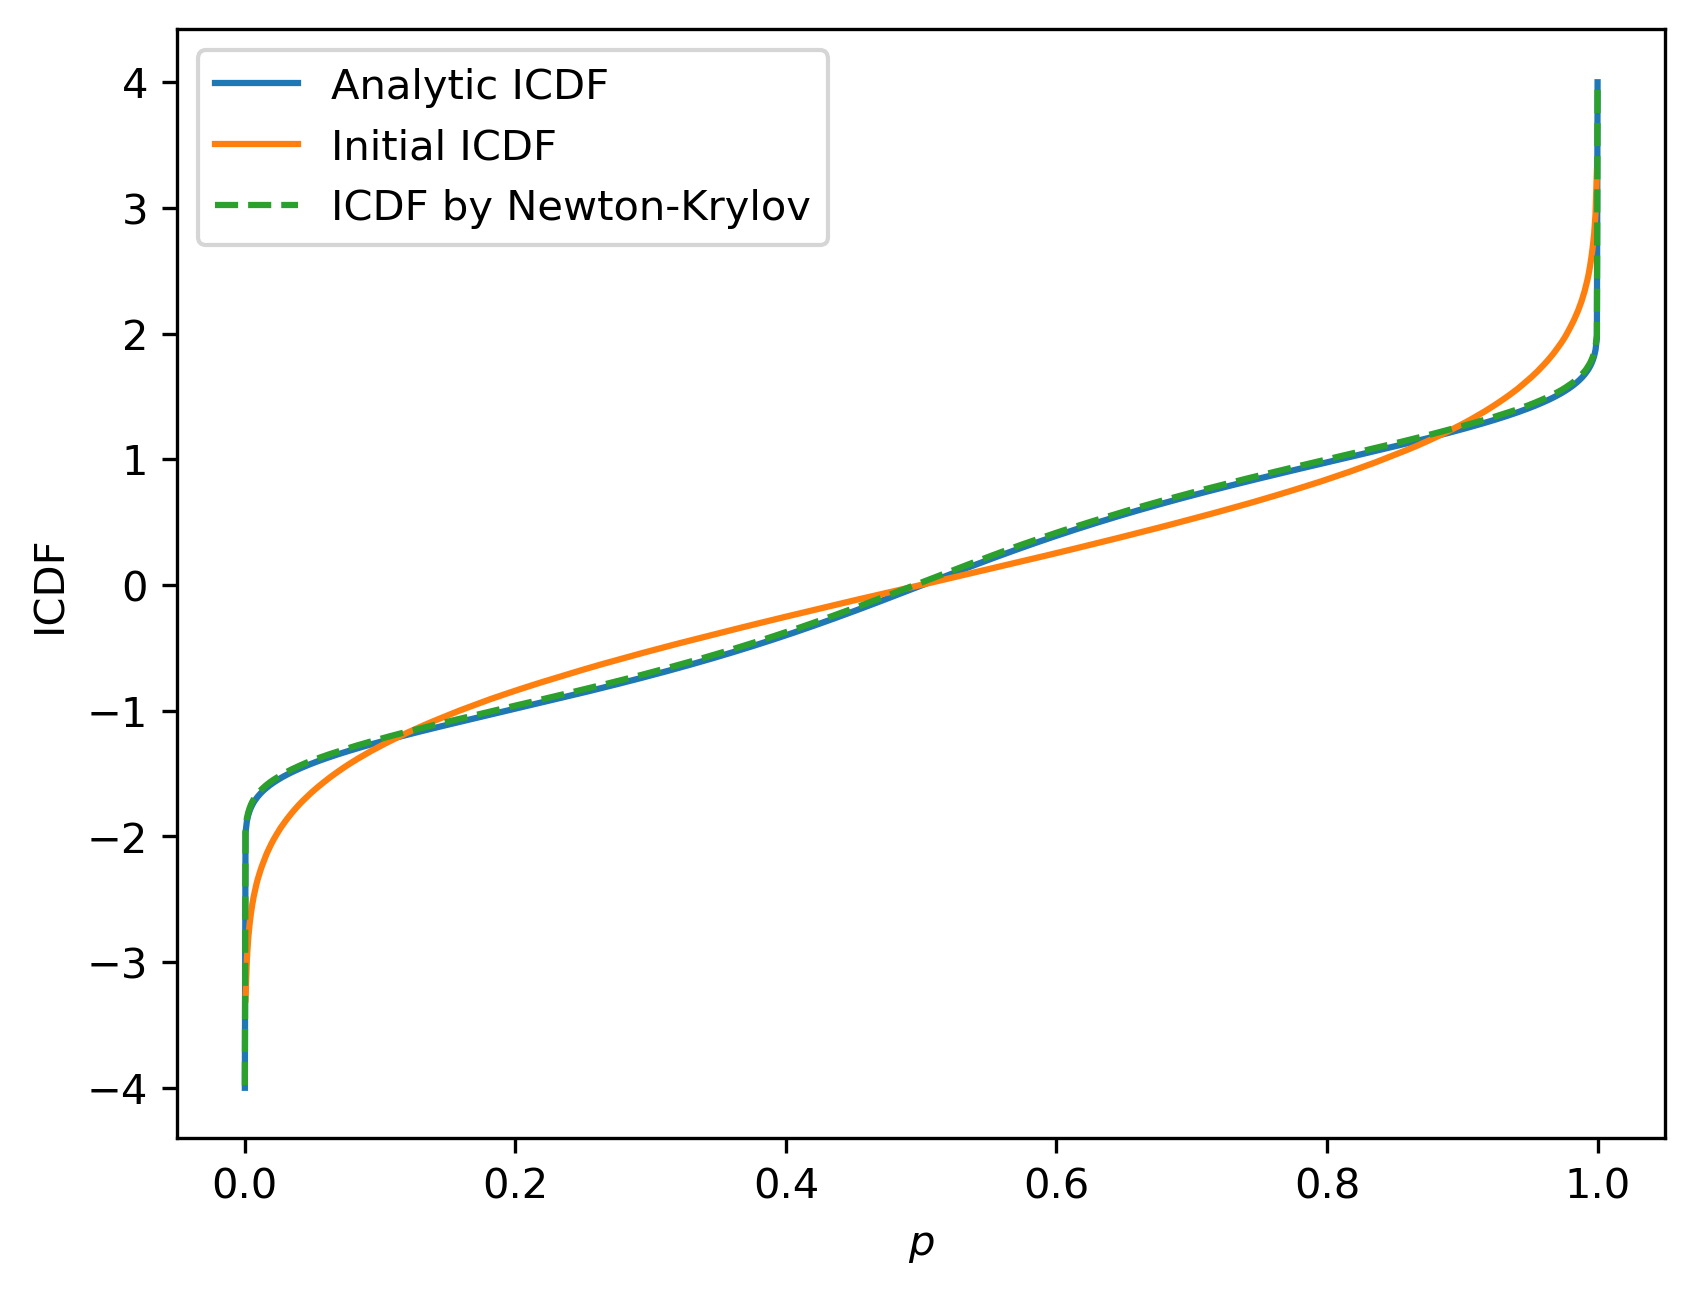
\includegraphics[width=\textwidth]{figures/ChemotaxisICDF.png}
    \end{subfigure}%
    \begin{subfigure}[b]{0.51\textwidth}
        \centering
        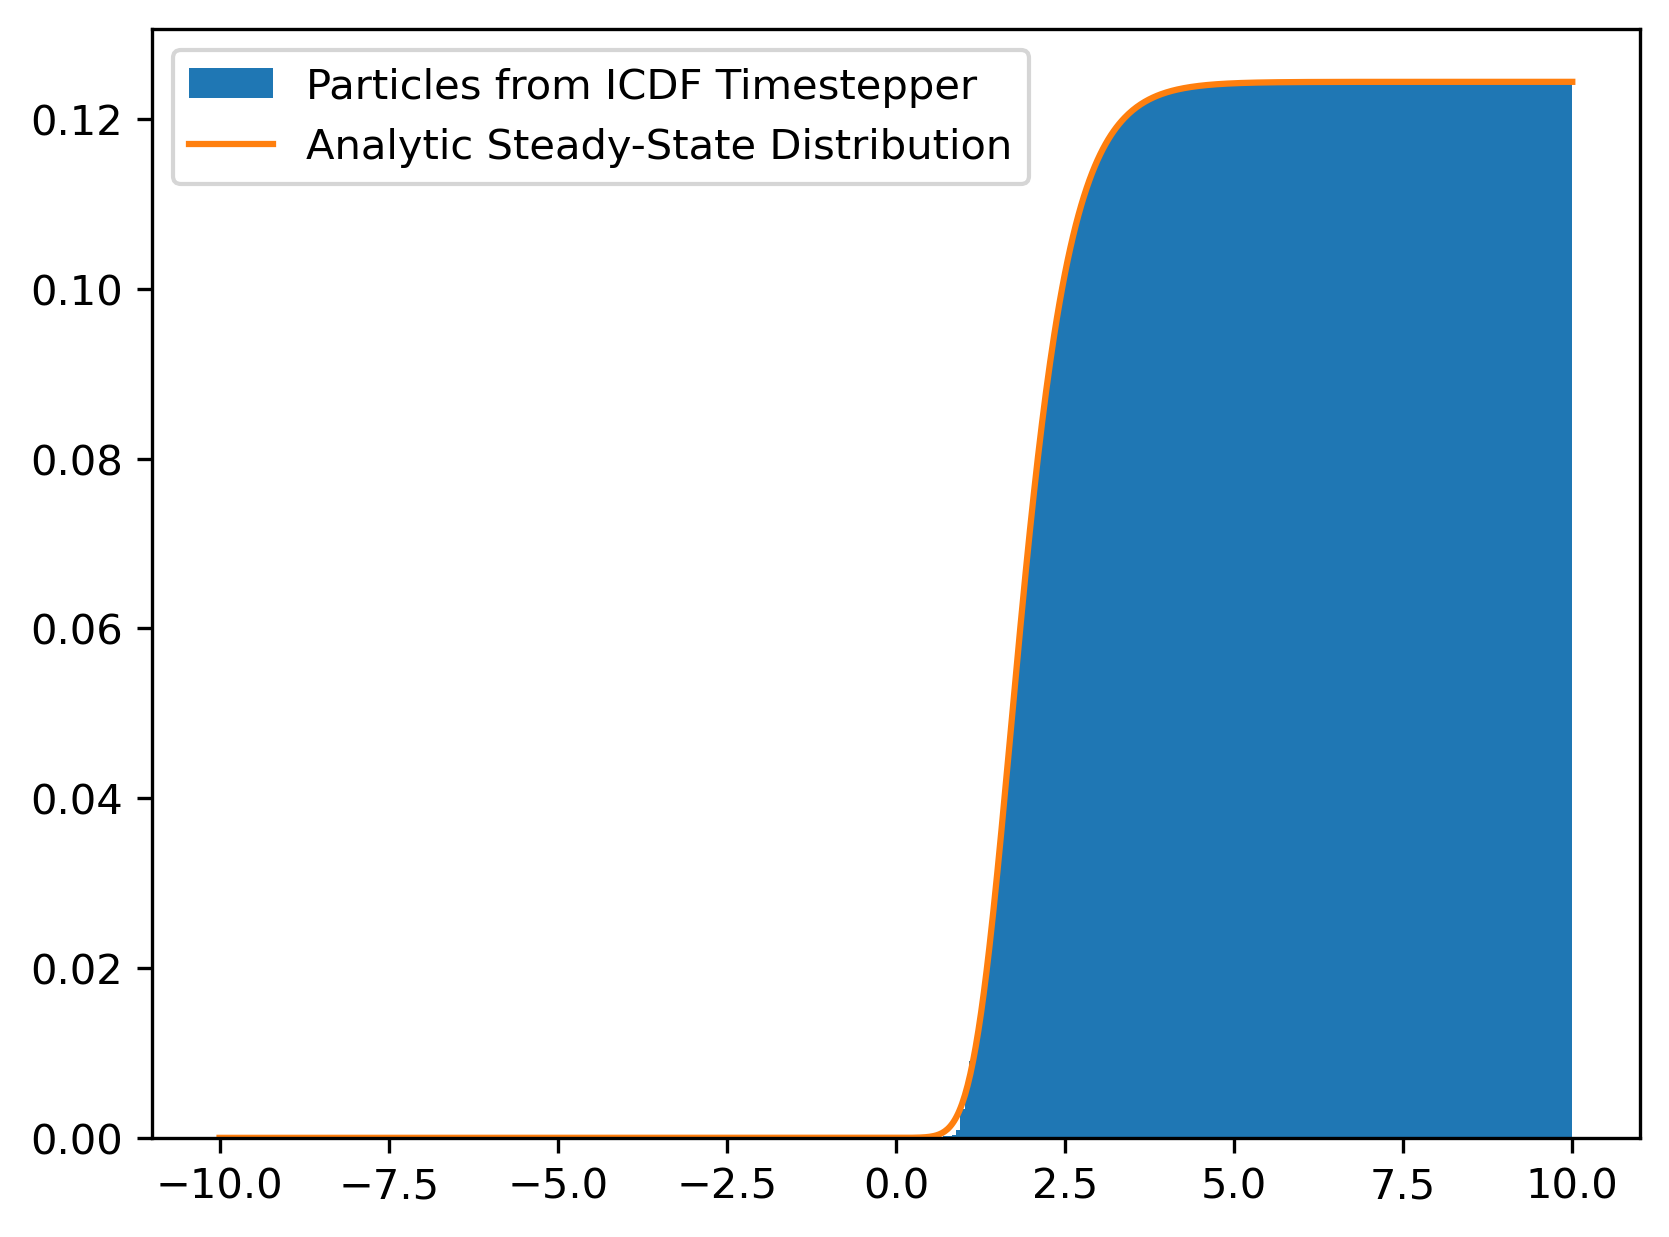
\includegraphics[width=\textwidth]{figures/ParticlesChemotaxisICDF.png}
    \end{subfigure}
    \caption{(Left) Initial (orange) true steady-state (blue) and steady-state ICDF computed by Newton-Krylov (dashed green). (Right) Particles sampled from the Newton-Krylov ICDF (blue) and corresponding steady-state density~\eqref{eq:chemotaxis_ss} in orange.}
    \label{fig:chemotaxis_icdf}
\end{figure}

Figure~\ref{fig:bimodal_icdf} illustrates the convergence of the Newton–Krylov method on this ICDF-to-ICDF timestepper. The left panel shows the initial ICDF (corresponding to the Gaussian guess), the true steady-state ICDF obtained from long-time simulation, and the ICDF recovered by Newton–Krylov. The latter two curves show close agreement, confirming that the method correctly identifies the stationary distribution. The right panel displays the histogram of $N = 10^5$ particles sampled from the steady-state ICDF computed by Newton–Krylov, which closely matches the invariant chemotactic density.

\subsubsection{Economic Agents}
As a final example, we apply the ICDF-to-ICDF timestepper framework to the economic agents model introduced in section~\ref{subsubsec:w2_agents}. The microscopic timestepper $\phi_T$ for this system is the McKean–Vlasov-type Euler scheme described in~\cite{fabiani2024task}. This model is nonlinear and non-local, and its corresponding mean-field equation~\eqref{eq:meanfield_agents} is known to admit multiple steady-state distributions.

The construction of the ICDF-to-ICDF timestepper is identical to the prior two examples. That is, we discretize the ICDF on a fixed percentile grid $p_k = (k - 0.5)/100$, for $1 \leq k \leq 100$ and $N = 10^5$ particles are sampled uniformly in percentile space. The microscopic timestepper $\phi_T$ is then applied to evolve these particles over a time horizon of $T = 1$ second. After propagation, the updated ICDF is reconstructed by sorting the particle ensemble retaining every $1000$th particle. The initial ICDF corresponds to a Gaussian distribution centered around $x = 0$ with standard deviation $0.1$. Jacobian–vector products of the timestepper are again computed using finite differences with step size $\varepsilon = 10^{-1}$.

\begin{figure}[h]
    \centering
    \begin{subfigure}[b]{0.51\textwidth}
        \centering
        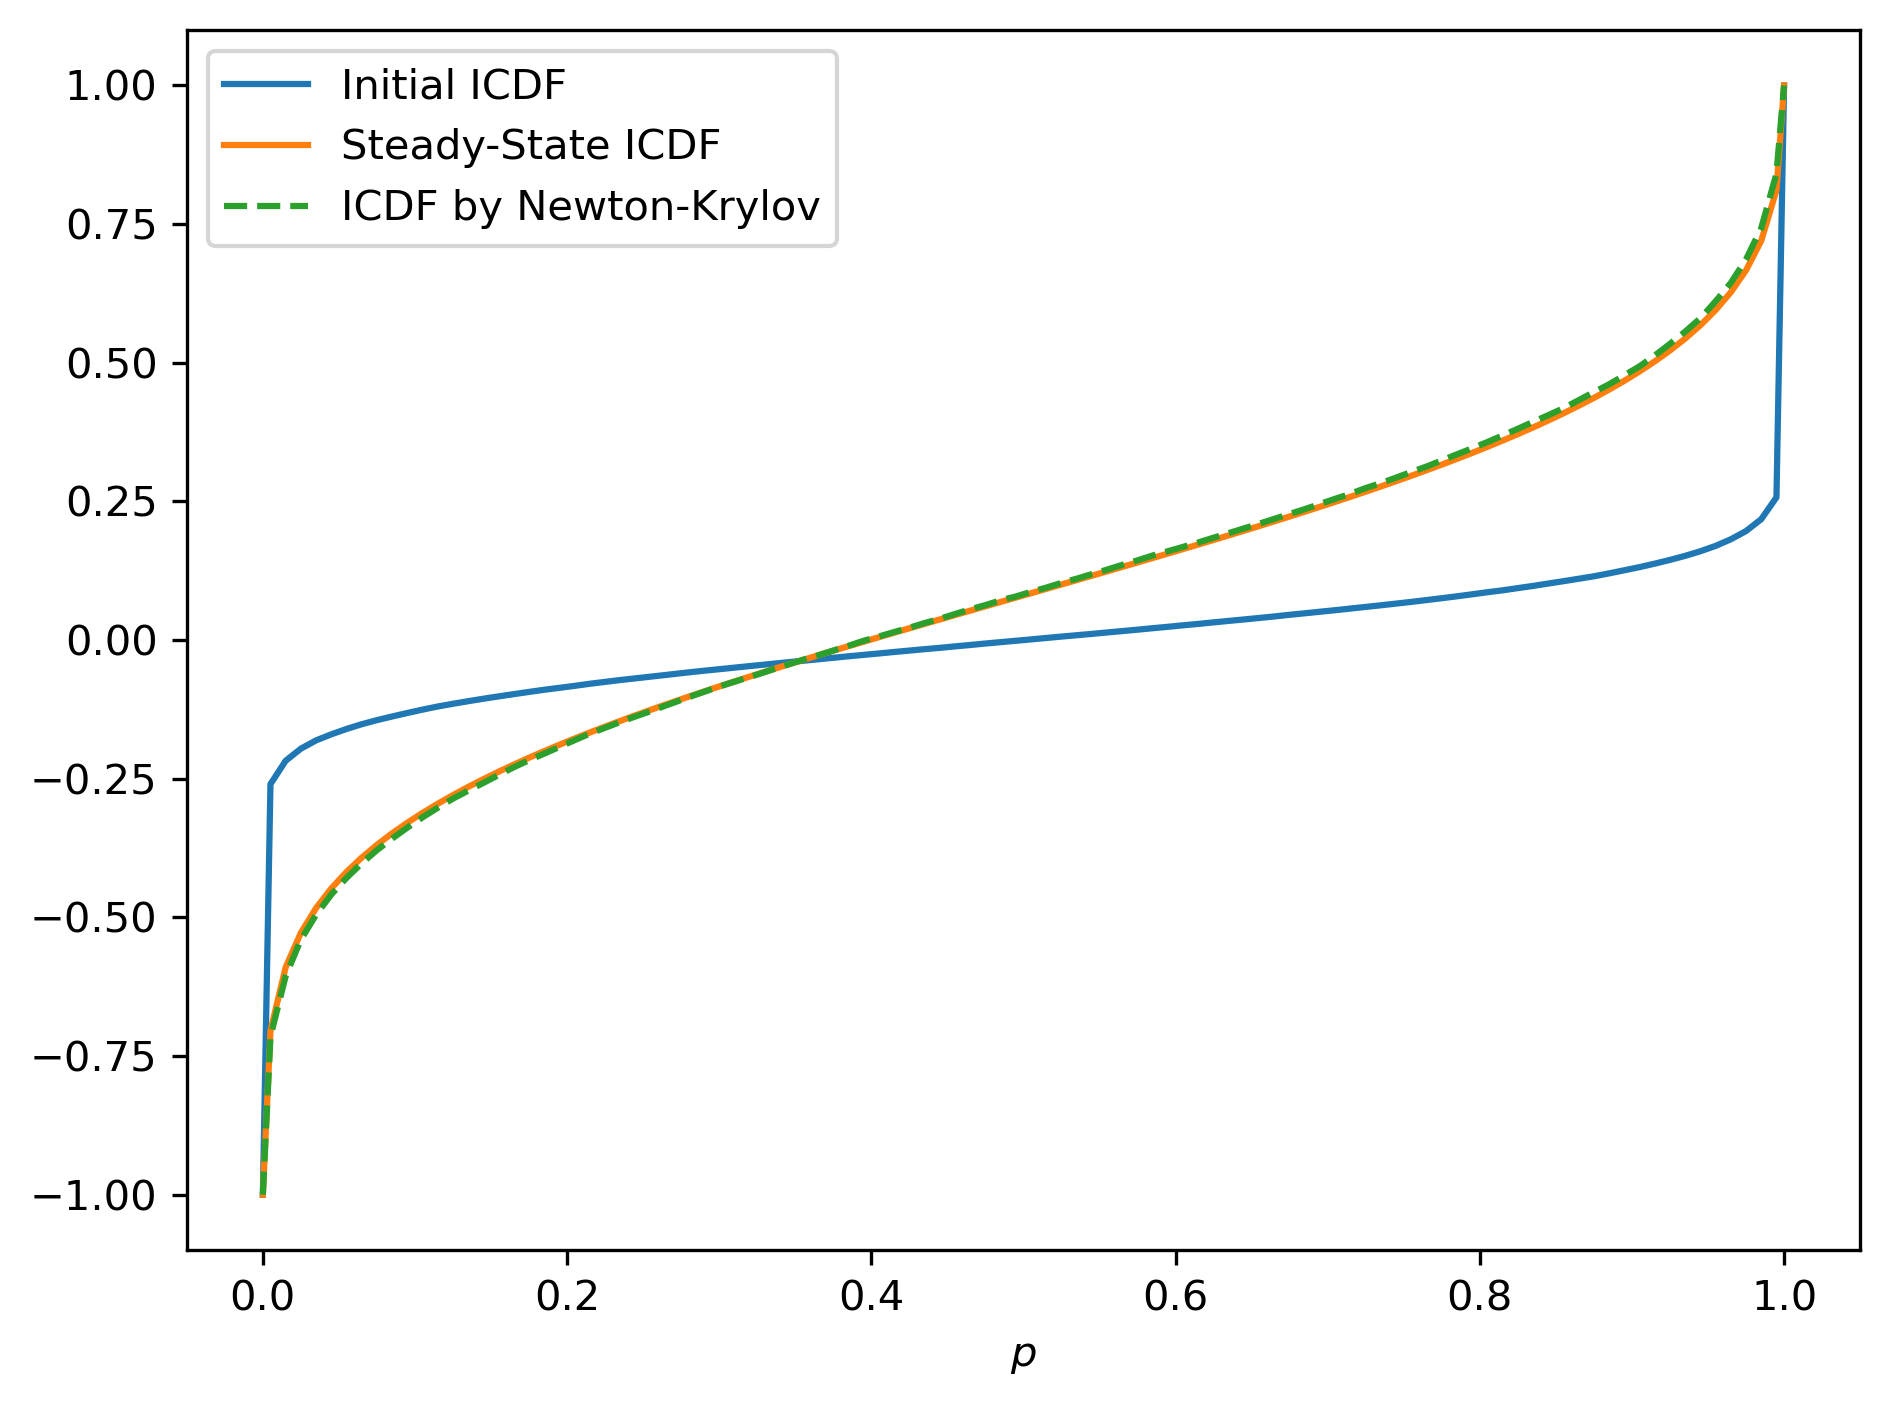
\includegraphics[width=\textwidth]{figures/EconomicsICDF.png}
    \end{subfigure}%
    \begin{subfigure}[b]{0.51\textwidth}
        \centering
        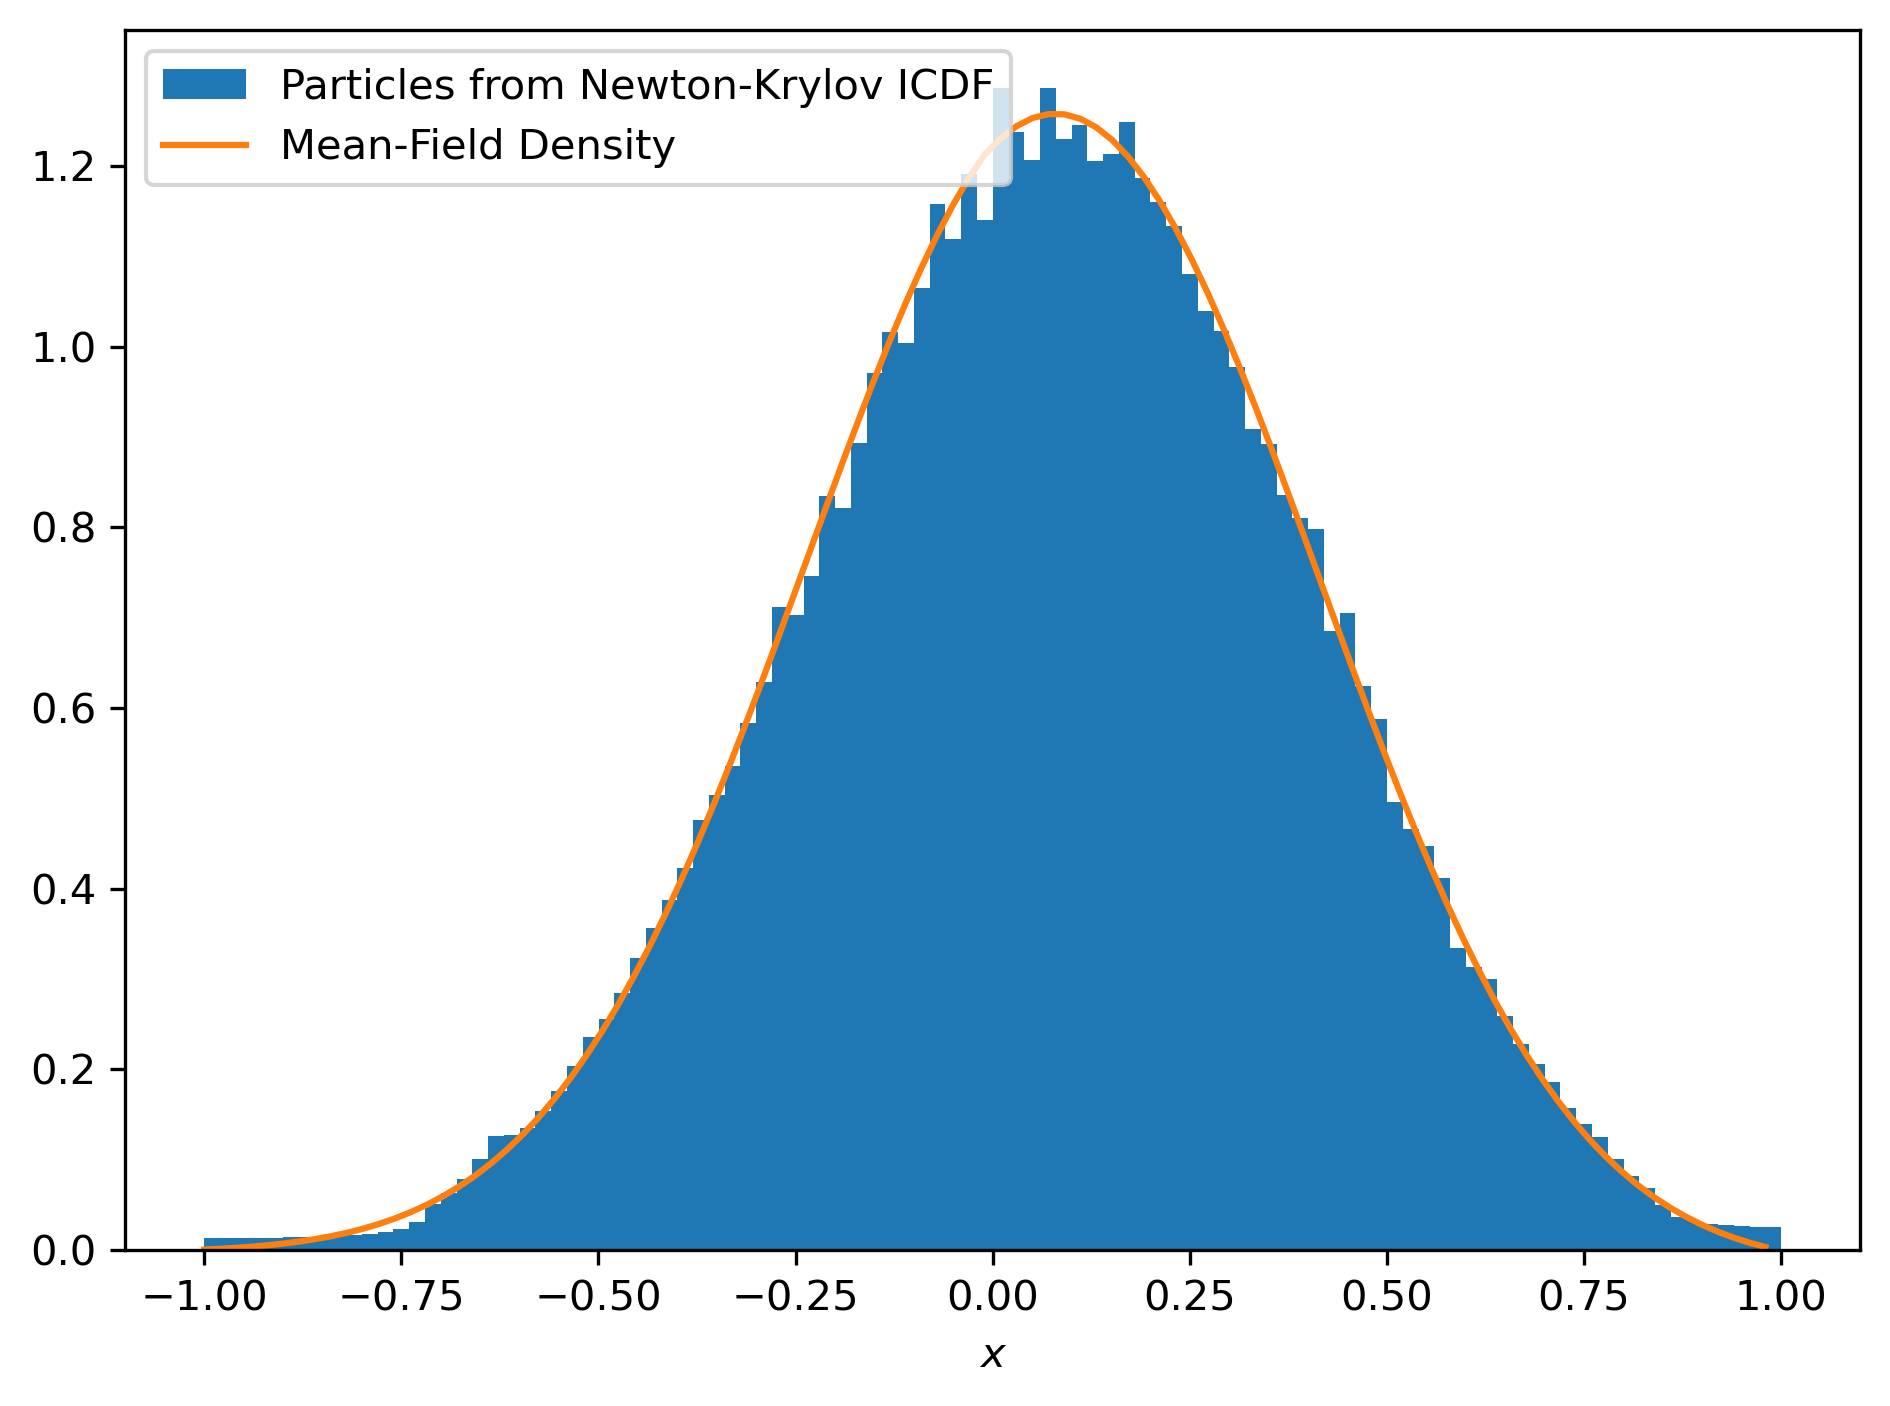
\includegraphics[width=\textwidth]{figures/EconomicsICDFParticles.png}
    \end{subfigure}
    \caption{(Left) Initial (blue) true steady-state (orange) and steady-state ICDF computed by Newton-Krylov (dashed green). (Right) Particles sampled from the Newton-Krylov ICDF (blue) and steady-state density corresponding to the mean-field PDE.}
    \label{fig:economics_icdf}
\end{figure}

Figure~\ref{fig:economics_icdf} illustrates the results obtained with Newton–Krylov on this ICDF timestepper. The left panel shows the initial ICDF, the invariant ICDF obtained from long-time microscopic simulation, and the steady-state ICDF recovered by Newton–Krylov. The close agreement between the two confirms that the algorithm correctly identifies the stable steady-state distributions of the system. The right panel displays the histogram of $N = 10^5$ particles sampled from the Newton–Krylov steady-state CDF, which closely matches the invariant distribution of the mean-field PDE~\eqref{eq:meanfield_agents}. 
\begin{figure}[h]
    \centering
    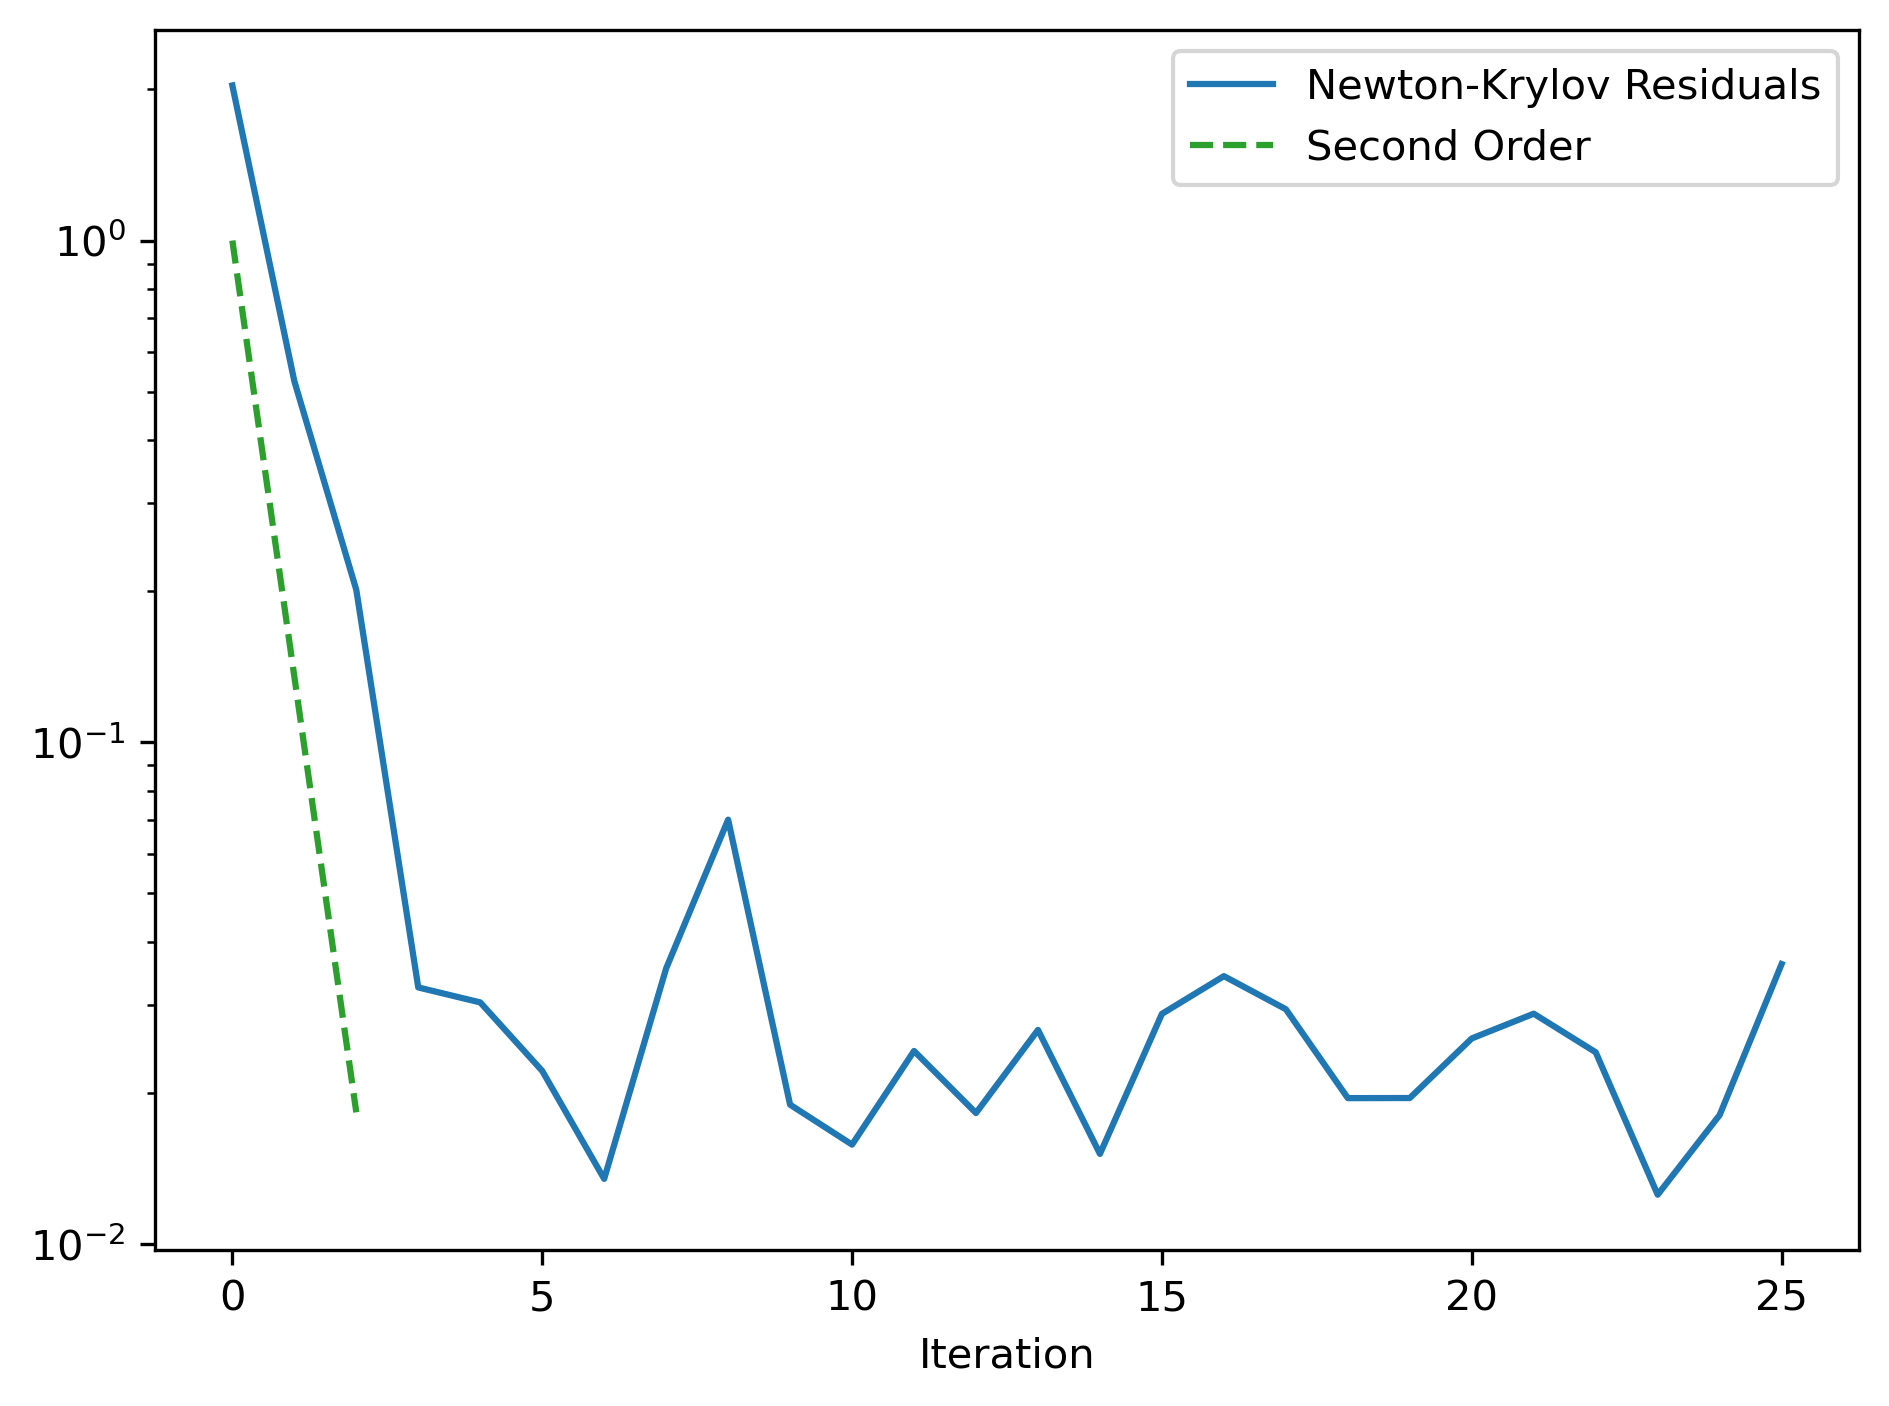
\includegraphics[width=0.6\textwidth]{figures/EconomicsICDFLosses.png}
    \caption{Newton-Krylov ICDF residual $\Psi\left((F^{-1})^{(k)}\right)$ per iteration for the economics agents model (blue); Second-order convergence rate (green). }
    \label{fig:economics_icdf_losses}
\end{figure}
For completeness we also show the Newton-Krylov error as a function of the iteration number in Figure~\ref{fig:economics_icdf_losses}. We see that the error first decreases quadratically as is typical for Newton-like schemes, before settling down in the noise regime.

\section{Extending Smooth Representations to Multiple Dimensions} \label{sec:higher_dimensions}
In contrast to the one-dimensional setting, an inverse cumulative distribution function cannot be defined in a straightforward manner for $d \ge 2$. The reason is that the CDF is not injective: for a given probability level $p \in [0,1]$, the level set
\begin{equation}
    \left\{(x,y) \in \mathbb{R}^2 | F_{X,Y}(x,y)=p\right\}
\end{equation}
typically forms a one-dimensional manifold (a curve) rather than a single point. Hence, the mapping $\left(F_{X,Y}\right)^{-1}(p)$ is not a well-defined function from $[0,1] \to \mathbb{R}^2$. Consequently, the notion of “evaluating the ICDF” becomes ambiguous in higher dimensions. It follows that the one-dimensional ICDF-based timestepper illustrated in Figure \ref{fig:icdftoicdf} cannot be extended to multivariate distributions in a direct manner. Even if a generalized notion of inverse CDF were introduced (e.g., by parameterizing level sets), its numerical evaluation would be computationally inefficient, since sampling points uniformly on such two-dimensional level sets is considerably more expensive than evaluating the scalar inverse $F^{-1}(p)$ in one dimension.

Alternatively, one may employ other smooth representations of particle distributions for calculating steady states of particle methods. We discuss two such alternatives in detail here: the multidimensional cumulative distribution function (section) and the sliced-Wasserstein distance. We discuss the former idea in section~\ref{subsec:cdf2d} and the latter in section~\ref{subsec:sw2}.

\subsection{The CDF-to-CDF Timestepper} \label{subsec:cdf2d}
A natural choice is to work directly with the two-dimensional cumulative distribution function $F_{X,Y}(x,y)$, which provides a continuous and differentiable description of the underlying particle ensemble. The notion of a cumulative distribution function (CDF) extends naturally to multiple dimensions. For clarity of exposition, we focus on the bivariate case, although all subsequent algorithms and results generalize to arbitrary dimension. Let $(X,Y)$ be a random vector with joint distribution. Its cumulative distribution function is defined by
\begin{equation}
 F_{X,Y}(x,y) = P(X\leq x, Y\leq y) = \int_{-\infty}^x \int_{-\infty}^y \mu(u,v) dudv.
\end{equation}

Sampling from a two-dimensional cumulative distribution function can be performed through its marginal and conditional components. Following the approach described by~\cite{}, the joint CDF $F_{X,Y}(x,y)$ can be decomposed into the marginal CDF $F_X(x)$ of one variable and the conditional CDF $F_{Y|x}(y|x)$ of the other. This decomposition allows sampling to proceed through a sequence of one-dimensional operations: one first draws a sample $x$ from the marginal cumulative distribution $F_X(x)$, and subsequently samples $y$ from the conditional cumulative distribution $F_{Y|X}(y)$. In this way, multidimensional sampling reduces to iterated evaluations of smooth one-dimensional ICDFs, which are mathematically well-defined.

The two-dimensional sampling algorithm works as follows. First we construct the marginal CDF of the $x$-coordinates, given by
\begin{equation}
    F_X(x) = P(X \leq x) = \int_{-\infty}^x \int_{-\infty}^{\infty} \mu(u,v) dudv = F_{X,Y}(x,\infty).
\end{equation}
This one-dimensional CDF can be easily inverted to generate samples $x_1, x_2, \dots, x_n$ at equidistant percentiles $p_i = (i-0.5)/n$. Next, for each $x$-sample $x_i$ we construct the one-dimensional CDF of the conditional distribution $\mu(y|x_i)$. It can be shown~\cite{} that this conditional cumulative distribution function is given by the formula
\begin{equation} \label{eq:conditional_cdf}
 F_{Y|X_i}(y) = \frac{\partial_x F_{X,Y}(X_i,Y)}{\mu_X(X_i)}.
\end{equation}
Given any smooth representation of $F_{X,Y}(x,y)$ this partial derivative is readily available, and sampling the $y$-coordinates $X_i$ can also be achieved by inverting $F_{Y|X_i}(y)$ and evaluating it in equidistant percentiles $q_j = (j-0.5)/m$. The end product of this staged sampling algorithm are $N$ particles $(X_n, Y_n)_{n=1}^N$. After propagating the particles through the timestepper
\begin{equation}
    (\tilde{X}_n,\tilde{Y}_n) = \phi_T(X_n,Y_n),
\end{equation}
we reconstruct the updated two-dimensional CDF by computing, at each grid node $(x_i, y_j)$, the fraction of particles $(\tilde{X}_n, \tilde{Y}_n )_{n=1}^N$ located in the lower-left quadrant relative to that point:
\begin{equation}
    F_{X,Y}(x_i,y_j) = \#\left\{ n \ | \ \tilde{X}_n \leq x_i \ \text{and} \ \tilde{Y}_n \leq y_j \right\} / N
\end{equation}
Starting from the CDF $F_{X,Y}^t$ at time $t$, the three steps 
\begin{itemize}
\item[1.] Sampling $(X_n,Y_n)$ from marginal and conditional CDFs; 
\item[2.] Forward particle propagation using the particle timestepper $(\tilde{X}_n, \tilde{Y}_n) = \phi_T(X_n, Y_n)$;
\item[3.] Restriction to the 2D CDF by counting particles in the lower right quadrant of each grid point;
\end{itemize}
define a consistent CDF-to-CDF timestepper
\begin{equation}
    \Phi_T\left(F_{X,Y}^t\right) = F_{X,Y}^{t+T}.
\end{equation}
See Figure~\ref{fig:cdftocdf} for a schematic of this timestepper. The associated residual map reads
\begin{equation} \label{eq:2dcdf_psi}
\Psi\left(F_{X,Y}^t\right) = F_{X,Y}^t - \Phi_T(F_{X,Y}^t),
\end{equation}
which is identical to $0$ at ever grid point $(x_i,y_j)$ in steady state. 

While constructing the two-dimensional CDF of a particle ensemble and re-sampling it through the marginal and conditional one-dimensional CDFs that we outlined above, provides a convenient way to generate new samples, this procedure is not equivalent to computing optimal transport (OT) map rearrangement of the original particles. Nonetheless, this algorithm yields a monotone triangular map that is close to the OT solution under many practical conditions. In fact, it corresponds to the Knothe–Rosenblatt rearrangement, a sequential, measure-preserving transformation that orders variables one at a time through their conditional distributions. While the Knothe–Rosenblatt map does not minimize the OT cost, it shares key structural properties and can be viewed as a computationally efficient approximation to the optimal transport map in high-dimensional sampling contexts. We do not require the exact optimal transport map in our Newton–Krylov calculations; any fast and reasonably accurate alternative that preserves the steady state is sufficient. The Knothe–Rosenblatt rearrangement offers a good alternative that is computationally efficient.

\begin{figure}[!ht]
  \centering
  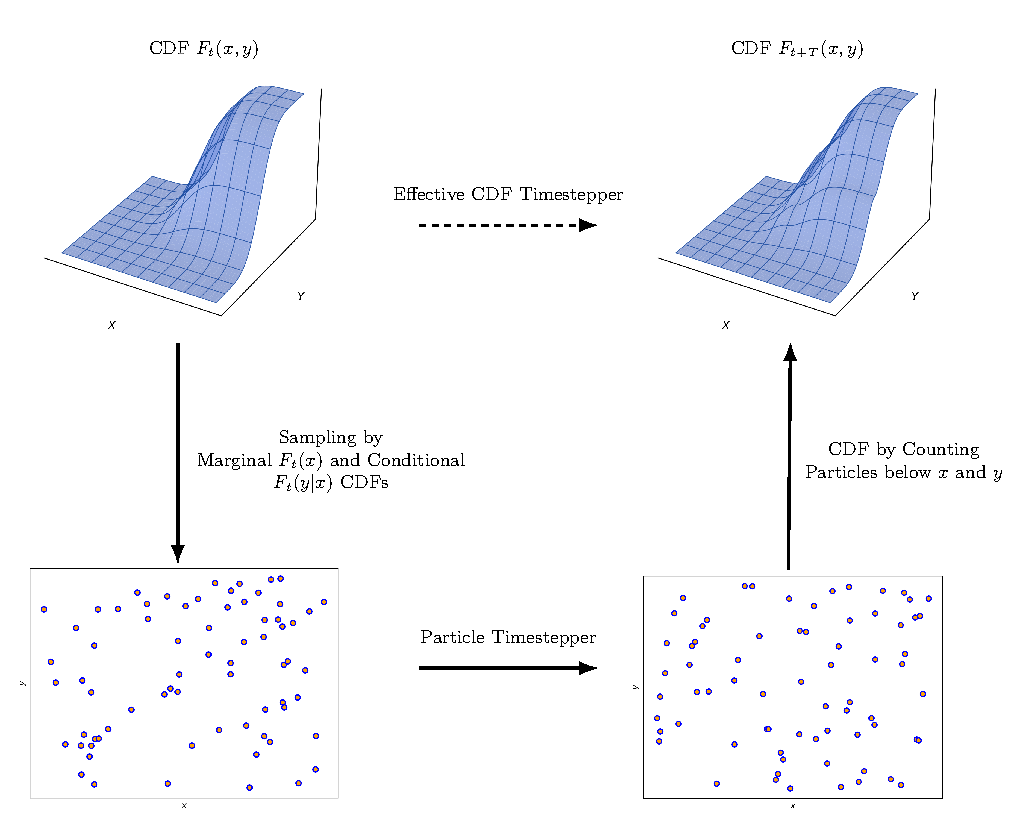
\includegraphics[width=0.8\textwidth]{CDFtoCDF.pdf}
  \caption{Schematic of the effective two-dimensional CDF–to-CDF timestepper.}
  \label{fig:cdftocdf}
\end{figure}

\paragraph{Numerical Example}
Consider the two-dimensional half-moon distribution~\eqref{eq:halfmoonpotential} as a representative example of our approach. We evaluate the empirical two-dimensional cumulative distribution function (CDF) on a uniform grid $(x_i, y_j)_{i,j}$ of $n_X = n_Y = 100$ points, equally spaced between $-4$ and $4$. The CDF-to-CDF timestepper is constructed using $N = 10^4$ particles, and sampling is performed by inverting the marginal and conditional one-dimensional cumulative distribution functions. To increase regularity, we interpolate the two-dimensional CDF with a piecewise-linear spline and solve for the corresponding percentiles. Specifically, for every percentile pair $(p_i, q_j)$, we determine the coordinates $(X_i, Y_j|X_i)$ such that
\begin{equation}
    F_X(X_i) = p_i, \ F_{Y|X_i}(Y_j) = q_j.
\end{equation}
This inversion can be implemented efficiently by vectorizing the evaluation of the marginal and conditional CDFs. Because the two-dimensional CDF is represented as a smooth spline, its partial derivatives—such as those appearing in~\eqref{eq:conditional_cdf}—are spline functions as well and need to be computed only once, independent of $p_i, q_j, X_i$ or $Y_j|X_i$.

We next apply the Newton-Krylov scheme to find the steady-state distribution of the CDF-to-CDF timestepper. The timestepper is based on an Euler-Maruyama discretization of the dynamics~\eqref{eq:langevin_halfmoon} with time step $\Delta t = 10^{-3}$. We integrate this dynamics up to time $T = 1$ second. The initial condition for the Newton-Krylov method is the standard bivariate Gaussian distribution (see the left of Figure~\ref{fig:nk_2dcdf}). 
\begin{figure}[h]
    \centering
    \begin{subfigure}[b]{0.51\textwidth}
        \centering
        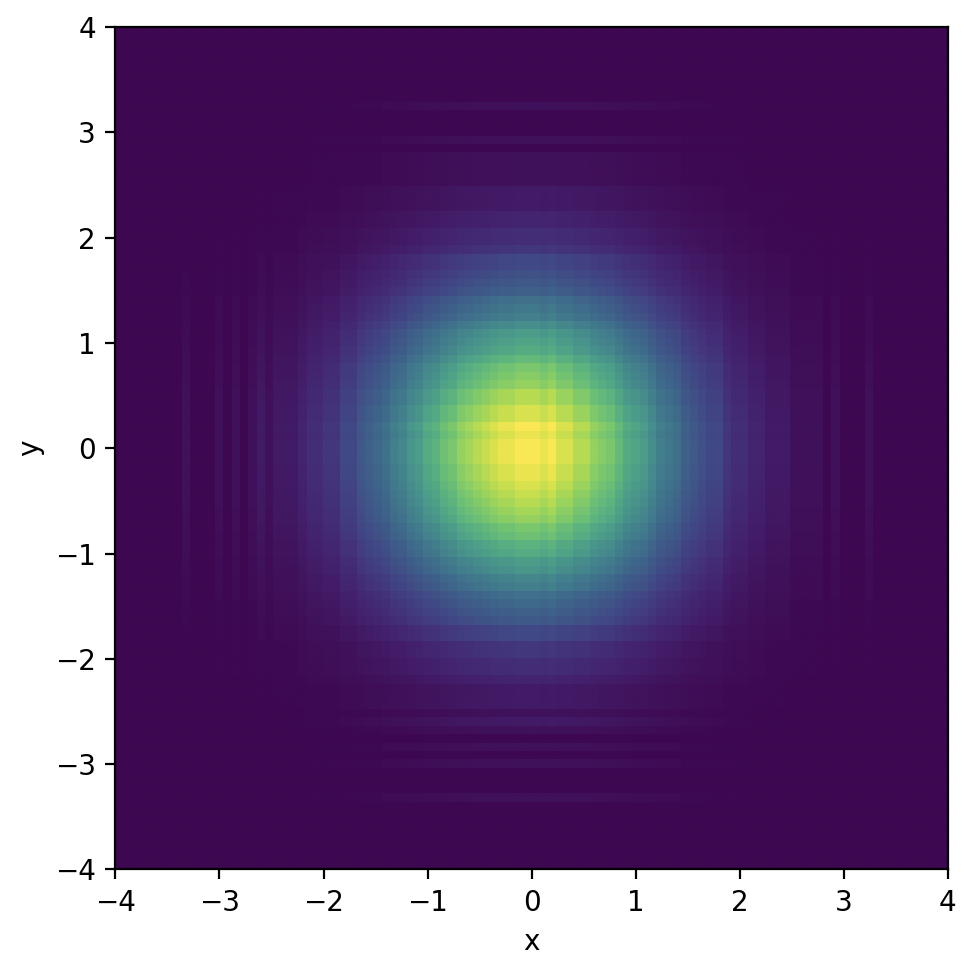
\includegraphics[width=0.852\textwidth]{figures/InitialGaussian.png}
    \end{subfigure}%
    \begin{subfigure}[b]{0.51\textwidth}
        \centering
        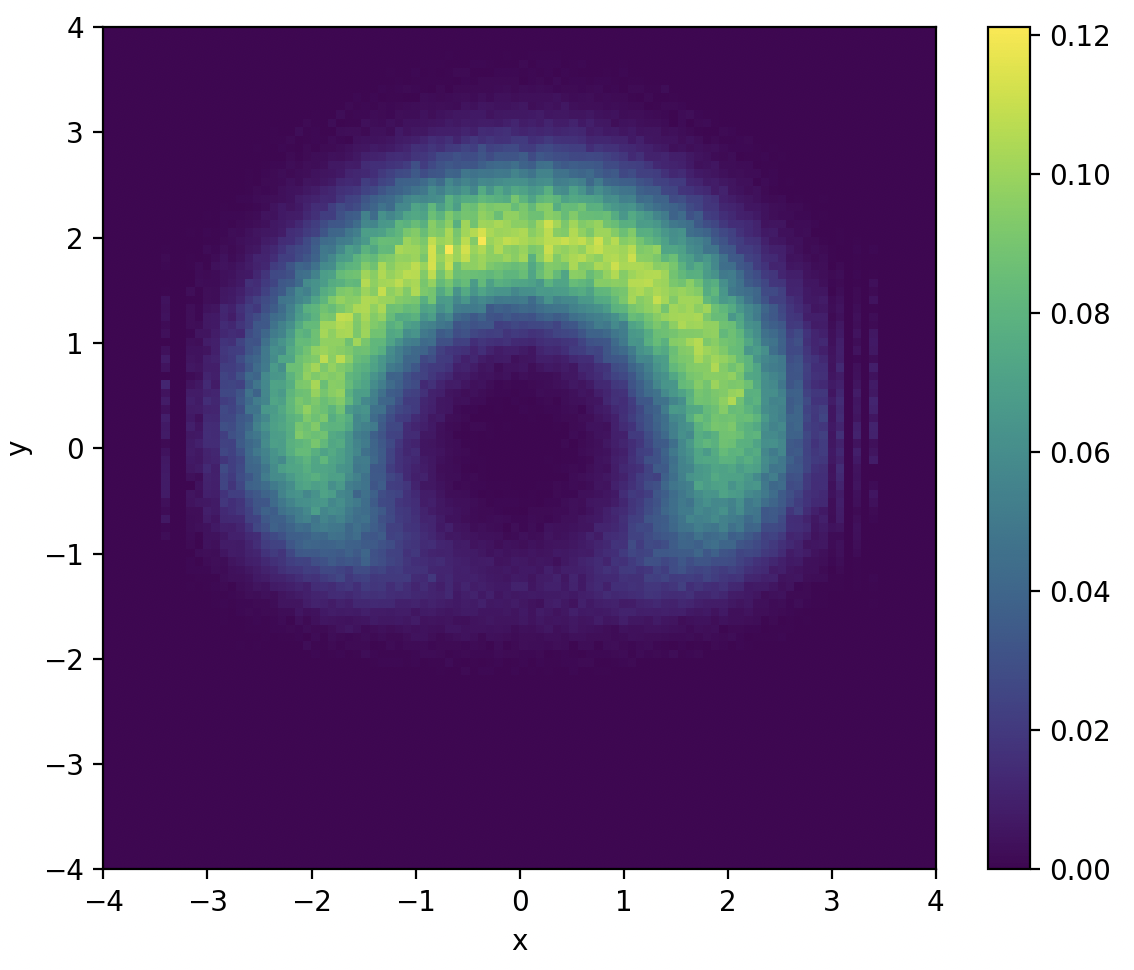
\includegraphics[width=\textwidth]{figures/CDF2DHalfMoon.png}
    \end{subfigure}
    \caption{Histogram heatmaps of particle density: (left) initial Gaussian condition; (right) distribution after Newton–Krylov optimization using the 2D CDF smooth representation.}
    \label{fig:nk_2dcdf}
\end{figure}
The optimized distribution obtained by Newton-Krylov is displayed on the right of Figure~\ref{fig:nk_2dcdf}. One can see that Newton-Krylov can recover the true steady-state distribution even though the initial distribution is quite far from equilibrium. Figure~\ref{fig:nk_2dcdf_loss} shows how the `loss` $\norm{\Psi\left(F_{X,Y}\right)}$ decreases steadily per nonlinear iteration and settles down to the noise level, a clear signal of convergence.

\begin{figure}[h]
    \centering
    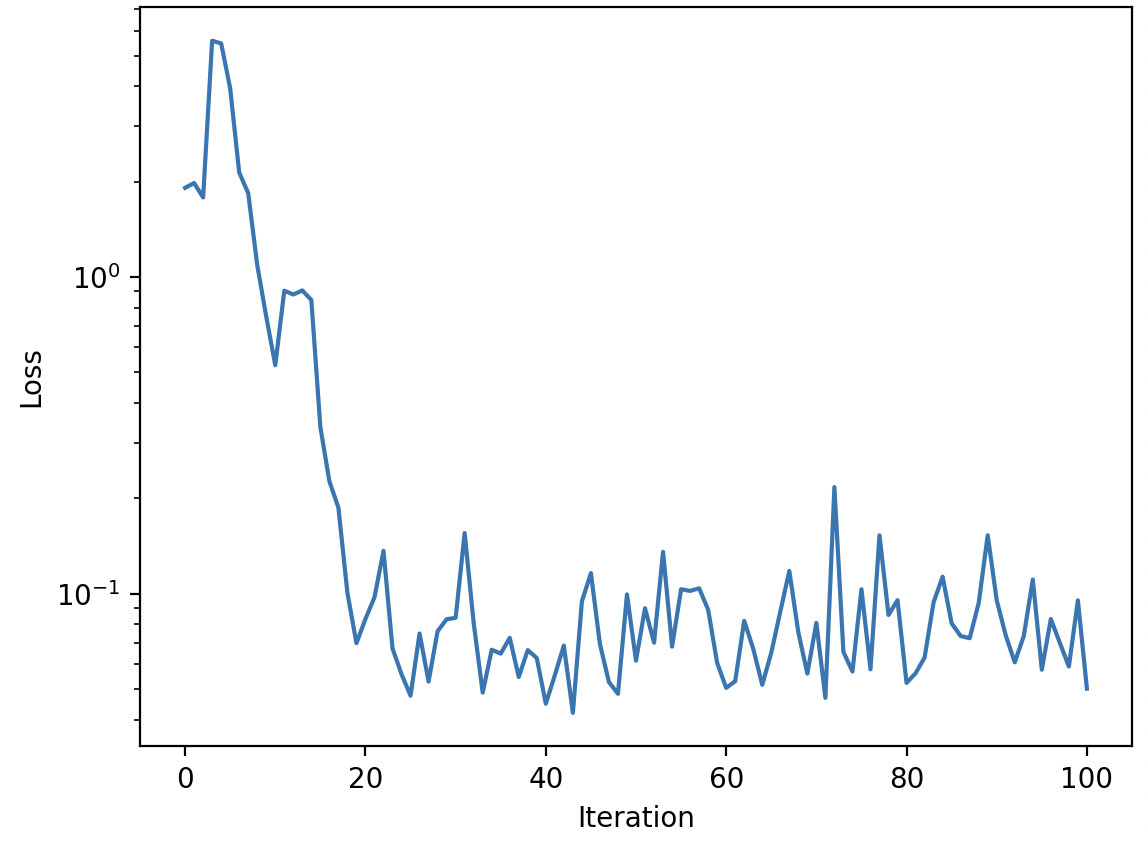
\includegraphics[width=0.5\textwidth]{figures/CDF2DHalfMoonLoss.png}
    \caption{Newton-Krylov loss $\norm{\Psi\left(F^{(k)}_{X,Y}\right)}$ per iteration $k$. The loss decreases up until a noise level induced by the finite number of particles.}
    \label{fig:nk_2dcdf_loss}
\end{figure}

\subsection{The Sliced Wasserstein Distance} \label{subsec:sw2}
For completeness, we also consider an alternative smooth representation of multidimensional particle systems based on the sliced Wasserstein distance (SWD). The key idea is to project probability distributions in $\mathbb{R}^d$ onto one-dimensional subspaces defined by unit vectors $\theta \in \mathbb{S}^{d-1}$ and to compute the Wasserstein distance between the resulting one-dimensional projected measures. Formally, for two distributions $\mu$ and $\nu$,
\begin{equation}
  SW_d^2(\mu,\nu) = \int_{\mathbb{S}^{d-1}}
  W_{d-1}^2\left(P_\theta \# \mu, P_\theta \# \nu\right)\,\mathrm{d}\theta,
\end{equation}
where $P_\theta(x)=\langle x,\theta\rangle$ is the projection onto the line spanned by~$\theta$ and $P_\theta \# \mu$ denotes the pushforward of $\mu$ by $P_\theta$.
In two dimensions, we approximate the integral with a finite set of angles $\{\theta_i\}_{i=1}^{N_\theta}$:
\begin{equation}
  SW_2^2(\mu,\nu)
  \;\approx\;
  \frac{1}{N_\theta}\sum_{i=1}^{N_\theta}
  W_2^2\!\big(P_{\theta_i}\#\mu,\; P_{\theta_i}\#\nu\big)
  \;=\;
  \frac{1}{N_\theta}\sum_{i=1}^{N_\theta}
  \int \!\big|F_{P_{\theta_i}\mu}^{-1}(r)-F_{P_{\theta_i}\nu}^{-1}(r)\big|^2\,\mathrm{d}r,
\end{equation}
where $F_{P_{\theta_i}\mu}$ is the one-dimensional CDF of the projected measure $P_{\theta_i}\#\mu$.

The sliced Wasserstein idea provides an alternative to build smooth timesteppers from an underlying particle timestepper. We retain a rectangular grid representation of the two-dimensional CDF, but sampling proceeds through directional projections. To achieve a consistent sampling, we need to first sample directions $\theta_i$ from the marginal angular CDF $F_\Theta$ and, for each $\theta_i$, generate radii $r_j|\theta_i$ from the conditional CDF $F_{R|\theta_i}(r)$. However, unlike the Cartesian marginal and conditional CDFs, there are no explicit expressions analogous to equations~\eqref{eq:marginal_cdf} and~\eqref{eq:conditional_cdf} for the marginal angular and conditional radial CDFs. We need to first explicitly construct the two-dimensional density
\begin{equation}
    \mu(x,y) = \nabla F_{X,Y}(x,y)
\end{equation}
which can be obtained efficiently from a spline representation of $F_{X,Y}$. Then the marginal angular CDF is given by
\begin{equation} \label{eq:marginal_angular}
    F_{\Theta}(\theta)
    = \int_{0}^{\theta} \int_{0}^{\infty}
        \mu \left(r \cos\phi,\, r \sin\phi\right)\,
        r\, dr\, d\phi.
\end{equation}
and the conditional radial CDF for any angle $\theta$ reads
\begin{equation} \label{eq:conditional_radial}
    F_{R|\theta}(r) = \int_{0}^{r} \mu(s \cos\theta, s\sin\theta)\ s\ ds.
\end{equation}
Sampling the 2D CDF consistently in a sliced Wasserstein-inspired way can then be achieved through
\begin{enumerate}
  \item Generate a set of angles $\{\theta_i\}_{i=1}^{N_\Theta}\subset[0,2\pi)$ by inverting the marginal angular CDF~\eqref{eq:marginal_angular} in fixed percentiles $p_i = (i - 0.5) / N_\Theta$;
  \item For each $\theta_i$, construct the radial conditional CDF $F_{R|\theta_i}(r)$ using the projection~\eqref{eq:conditional_radial}.
  \item Invert each radial conditional CDF in fixed percentiles $\{r_j\}_{j=1}^{N_r}\subset(0,1)$ through a bisection-like scheme
        \[
          \rho_{ij} \;=\; F_{R | \theta_i}^{-1}(r_j).
        \]
  \item Map these 1D samples back to $\mathbb{R}^2$ via the inverse projection
        \[
          X_n=\rho_{ij}\cos\theta_i, \qquad Y_n=\rho_{ij}\sin\theta_i,
        \]
        and collect all $(X_n,Y_n)$ across $i,j$.
\end{enumerate}
After sampling we proceed as with the CDF-to-CDF timestepper by propagating the samples through the particle timestepper to obtain new particles $(\tilde{X}_n,\tilde{Y}_n)$ and restricting back to the CDF by counting the number of $(\tilde{X}_n,\tilde{Y}_n)$ to the lower left of each CDF grid point $(x_i,y_j)$. Together, this sliced representation captures much of the transport geometry while remaining computationally light, providing a scalable surrogate for the full multidimensional Wasserstein map within our Newton-Krylov framework. The complete sliced Wasserstein-to-sliced Wasserstein timestepper is shown schematically in Figure~\ref{fig:swtosw}. 

\begin{figure}[!ht]
  \centering
  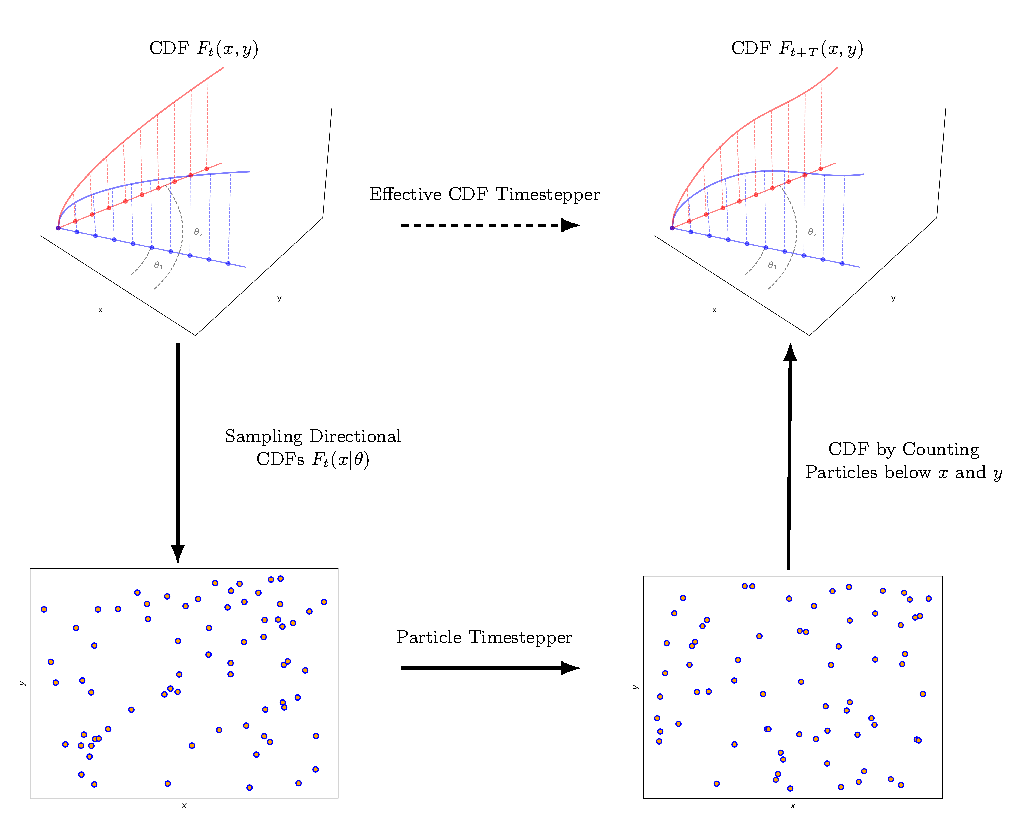
\includegraphics[width=0.8\textwidth]{SWtoSW.pdf}
  \caption{Schematic of the effective sliced Wasserstein to sliced Wasserstein timestepper.}
  \label{fig:swtosw}
\end{figure}

Finally we also show how the Newton-Krylov method on the sliced-Wasserstein representation of particles converges to the steady-state distribution of the half-moon potential. The initial condition and timestepper parameters are the same as in section~\ref{subsec:cdf2d}, and sampling is done by first generating $N_\Theta=100$ angular samples and then $N_R=100$ radial samples for each angle. The Newton-Krylov loss per iteration is shown in the left subfigure of Figure~\ref{fig:nk_sw2} and the resulting steady-state distribution is shown on the right.

\begin{figure}[h]
    \centering
    \begin{subfigure}[b]{0.5\textwidth}
        \centering
        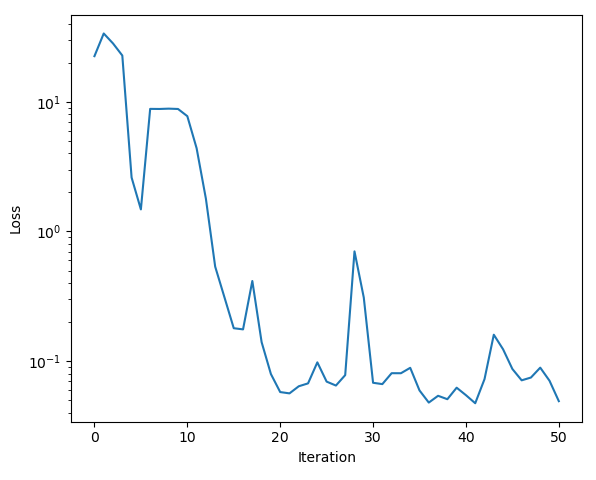
\includegraphics[width=\textwidth]{figures/SWLoss.png}
    \end{subfigure}%
    \begin{subfigure}[b]{0.5\textwidth}
        \centering
        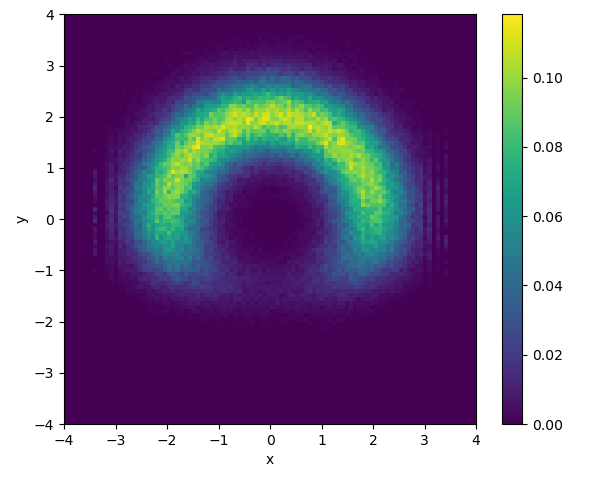
\includegraphics[width=\textwidth]{figures/SW Heatmap.png}
    \end{subfigure}
    \caption{(left) Loss $\norm{\Psi(F_{X,Y}^{(k)}}$ per iteration; (right) Histogram heatmap of resulting steady-state particle density of the Newton-Krylov method applied to the Sliced Wasserstein representation.}
    \label{fig:nk_sw2}
\end{figure}

As shown, there is no significant difference in either the convergence rate or the resulting steady state between the sliced Wasserstein and the direct CDF representations. This outcome is expected, since both formulations are mathematically equivalent. The key insight is that employing smooth representations enables the use of higher-order optimization schemes, while the specific choice of representation is comparatively unimportant. The decisive factor is the computational efficiency of sampling.

\section{Discussion and Outlook} \label{sec:conclusion}
We have presented a unified, matrix-free framework for computing steady-state distributions of particle timesteppers. The key idea is to reformulate a steady state in the language of optimal transport. On the deterministic side, we revisited the residual formulation $\psi(u) = u - \phi_T(u)$ and showed how the Newton–Krylov method efficiently recovers steady states of the Fokker-Planck equation. We also derived a practical criterion for selecting the integration horizon $T$ from the spectral gap. On the stochastic side, we a first-order Adam-Wasserstein method for calculating steady states directly on the particle level. We also clarified why a naive particle-level extension fails to higher-order optimizers such as Newton-Krylov. Stochastic noise breaks the one-to-one correspondence between ensembles, and Jacobian–vector products acquire variance scaling as $1/\varepsilon$. Our analysis makes this bias–variance trade-off explicit and shows that stable convergence can be achieved when the finite-difference step size is chosen within a noise-dependent range.

To address this limitation, we introduced smooth distributional timesteppers—first in one dimension through the ICDF-to-ICDF map, and then in multiple dimensions through CDF-to-CDF and sliced Wasserstein formulations. These representations aggregate microscopic variability into smooth macroscopic objects on which Newton–Krylov regains its fast, second-order convergence. Numerical results confirm that these smooth timesteppers yield comparable steady states with markedly reduced stochastic fluctuations, enabling accurate steady-state computations even in noisy particle systems. The central message is that smoothness in representation, rather than in the underlying dynamics, is the key to robust, matrix-free solvers for stochastic steady states.

One the main questions we want to address during further research will be to reduce the stochastic error in the finite-differences approximation of the Jacobian. Variance reduction at the particle level through correlated samples could further stabilize Jacobian-vector products and allow smaller finite-difference steps. In the case of central finite differences, antithetic variables might be a natural variance reduction technique. 

Beyond computing single steady states, an important next step is to apply Newton-Krylov to compute steady-state branches of parameter-dependent particle systems. Such numerical continuation algorithms require consistent residual evaluations between successive Newton–Krylov steps. Therefore, improving variance reduction at the particle level—through correlated sampling, common-random-number strategies, or smoother estimators will be crucial for enabling robust and efficient continuation of stochastic steady states, including the reliable detection of folds and bifurcations in distribution space.

Finally, scaling these approaches to large particle ensembles and to systems with potentially thousands of dimensions remains a major challenge. A key open question is how to identify the most effective sampling strategy for multidimensional CDFs (or their smooth equivalents) constructed via percentile evaluations. What constitutes “best” in this context is not yet defined, but it will likely involve a balance between proximity to the true optimal transport map (much like the Knothe–Rosenblatt rearrangement approximates it) and the computational efficiency of the resulting sampling algorithm. Establishing this balance will be essential for extending smooth timestepper frameworks to high-dimensional stochastic systems like molecular dynamics or real economic systems.

\textbf{[Anything else you are thinking of?]}

\appendix
\section{Derivation of the Relation between the Eigenvalues of $Df$ and $D\phi_T$} \label{app:eigenvalues}
Let 
	\begin{equation} \label{eq:pde}
		\partial_t u_t = f\left(u_t\right)
	\end{equation}
	be a semi-discretized PDE. We are interested in steady-state points $u^*$ such that $f(u^*)=0$. However, in most situations the right-hand side $f$ of the PDE is not available, only a timestepper is. Call $\phi_T(u)$ the flow map of a timestepper with initial condition $u$ over a time interval of size $T$. Steady-states of the PDE~\eqref{eq:pde}, i.e., zeros of $f$, are also zeros of
	\begin{equation}
		\psi(u) = u - \phi_T(u).
	\end{equation}
	Additionally, stable steady states of $f$ are stable steady states of $\psi$ and vise versa. In general, the following theorem holds.
	\begin{theorem}
		Let $\lambda_i$ and $\mu_i$ be the respective eigenvalues of $D f(u^*)$ and $D \phi_T(u^*)$. Then $\mu_i = \exp\left(\lambda_i T\right)$. 
	\end{theorem}
	\begin{proof}
		Starting from the integral representation of ODE~\eqref{eq:pde},
		\begin{equation*}
			\phi_T(u) = u + \int_{0}^{T} \partial_s u_s ds = \int_{0}^{T} f\left(u_s\right) ds.
		\end{equation*}
		Then, taking the gradient with respect to the initial condition $u$ ($D=D_u$), we get
		\begin{equation} \label{eq:integral_nabla_phi}
			D \phi_T(u) = I + D_u \int_{0}^{T} f\left(u_s\right) ds = I + \int_{0}^{T} D \left[f\left(u_s\right) \right]ds.
		\end{equation}
		Applying the chain rule $D \left[f\left(u_s\right) \right] = D f\left(u_s\right) D u_s$. However, $u_s$ is just $\phi_s(u)$. Plugging these results into equation~\eqref{eq:integral_nabla_phi}
		\begin{equation*}
			D \phi_T(u) = I + \int_{0}^{T} D f\left(u_s\right) D \phi_s(u) ds.
		\end{equation*}
		For brevity, call $J(s) = D f(u_s)$ and $A(t) = D \phi_t(u)$. We then obtain a compact integral equation
		\begin{equation*}
			A(t) = I + \int_{0}^{T} J(s) A(s) ds,
    	\end{equation*}
    	which is the integral representation of the solution to the matrix ODE
    	\begin{equation} \label{eq:matrix_ode}
    		\partial_t A(t) = J(t) A(t)
    	\end{equation}
	   with initial condition $A(0)=I$. This ODE has a unique solution
    	\begin{equation*}
    		A(t) = \exp\left(\int_{0}^t J(s) ds\right).
    	\end{equation*}
	   In steady-state, $J(s)$ is just a constant matrix $J=D f(u^*) $, and $A(t) = \exp\left(t J \right) $. The eigenvalues of $J$ are just $\lambda_i$.  We can conclude that the eigenvalues of $D \phi_T(u^*)=A(T)$ are $\exp\left(T \lambda_i \right)$, and therefore
	\begin{equation*}
		\mu_i = 1- \exp\left(T \lambda_i \right).
	\end{equation*}
\end{proof}

\section{Analytic Steady-State Distribution of the Chemotaxis Model} \label{app:chemotaxis}
The chemotaxis stochastic model~\eqref{eq:chemotaxis} can be seen as a special case of the overdamped Langevin dynamics
\begin{equation}
    dX_t = -U'(X_t) dt + \sqrt{2 D} dW_t
\end{equation}
with potential energy 
\begin{equation*}
U(x) = -\int_{-L}^x \chi(S(y)) S_y(y) dy = -\int_{S(-L)}^{S(x)} \chi(S)dS.
\end{equation*}
The invariant distribution of the overdamped Langevin dynamics is
\begin{equation*}
    \mu(x) = Z^{-1} \exp\left(-\frac{1}{D} U(x)\right) = Z^{-1} \exp\left(\frac{1}{D} \int_{-1}^{S(x)} \chi(S)dS\right)
\end{equation*}
It can be seen that the no-flux boundary conditions are automatically satisfied because $J(x) = 0$ everywhere in steady state.
\bibliographystyle{plain}
\bibliography{references.bib}

\end{document}
